\documentclass[11pt]{book}

\usepackage{xcolor}
\usepackage{fontspec}
\setmainfont[
Path = fonts/, 
UprightFont = TitilliumWeb-Regular.ttf,
BoldFont = TitilliumWeb-Bold.ttf,
ItalicFont = TitilliumWeb-Italic.ttf,
BoldItalicFont = TitilliumWeb-BoldItalic.ttf
]{TitilliumWeb}

%\usepackage[utf8]{inputenc}
%\usepackage{listingsutf8}
%\lstset{inputencoding=utf8}

\usepackage{tabularx}
\usepackage[a4paper,outer=3cm,inner=3cm,top=3cm,bottom=3cm]{geometry}
\usepackage[colorlinks=true, linkcolor=black, citecolor=blue, urlcolor=blue]{hyperref}
\usepackage{graphicx}
\usepackage{xcolor}
\graphicspath{{images/}}
\usepackage{listings}
\usepackage{svg}

\usepackage{tikz}
\usetikzlibrary{shapes.geometric, arrows.meta, positioning}

\newcommand{\authors}[1]{{\chapterauthor{#1}\addtocontents{toc}{#1\par}}}
\newcommand{\HUGE}{\fontsize{40}{48}\selectfont}

\renewcommand{\contentsname}{Daftar Isi}
\renewcommand{\chaptername}{Bab}
\renewcommand{\figurename}{Gambar}

\makeatletter
\newcommand{\chapterauthor}[1]{%
	{\parindent0pt\vspace*{-25pt}%
		\linespread{1.1}\large\scshape#1%
		\par\nobreak\vspace*{35pt}}
	\@afterheading%
}
\makeatother

\begin{document}


\begin{titlepage}
	\begin{tikzpicture}[remember picture, overlay]
		% Gambar latar belakang atau logo
		\node[anchor=north west, inner sep=0pt] at ([xshift=.18\textwidth, yshift=-.1\textwidth] current page.north west){
			
\includegraphics[width=.3\paperwidth]{../figures/logo_universitas.png} 
		};
	
		\node[anchor=north west, inner sep=0pt, opacity=.12] at (current page.north west){
			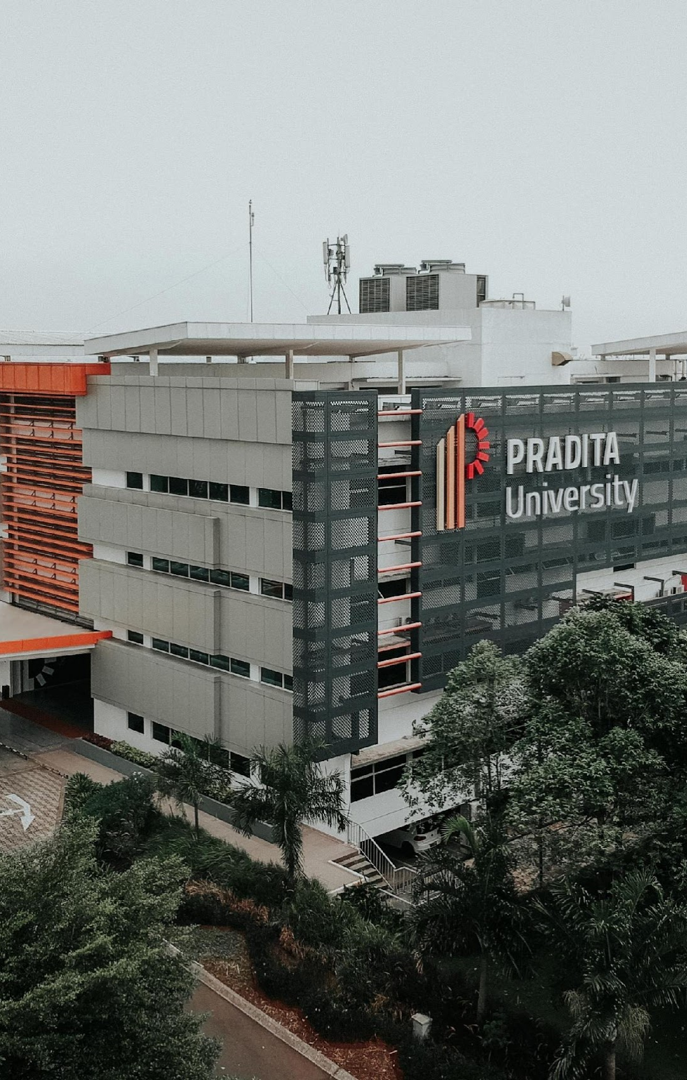
\includegraphics[width=\paperwidth]{../figures/building.png}
		};
		
		% Judul Tengah
		\node[anchor=center] at ([yshift=.1\textheight]current page.center) {
			\begin{minipage}{\textwidth}
				
				{\LARGE \textbf{Buku Ajar}}\\[0.03\textheight] % Book Type
				{\HUGE \textcolor{orange}{\textbf{Pelatihan AI untuk Guru}}}\\[.04\textheight] % Title
				{\Huge \textcolor{orange}{\textbf{Penggunaan Large-language Model}}}\\[.08\textheight] % Subtitle
				{\LARGE \textbf{Alfa Yohannis}}\\[0.05\textheight] % Authors
			\end{minipage}
		};
		
		% Teks bawah dengan latar oranye penuh dan teks putih
		\node[anchor=south west] at (
		current page.south west) {
			\begin{tikzpicture}[remember picture, overlay]
				\node[anchor=south west, fill=orange, text=white, minimum width=\paperwidth, minimum height=.14\textheight, align=center, font=\Huge\bfseries] at (-.15,-.15) {
					Program Studi Informatika\\
					Pradita University
				};
			\end{tikzpicture}
		};
	\end{tikzpicture}
\end{titlepage}
	
	% Contents Page
	\tableofcontents
	
	\chapter{Pendahuluan}

Perkembangan teknologi kecerdasan buatan (AI) telah menghadirkan perubahan signifikan da\-lam berbagai aspek kehidupan, termasuk dunia pendidikan. Salah satu inovasi yang paling menonjol dalam beberapa tahun terakhir adalah kemunculan \textit{Large Language Model} (LLM) se\-per\-ti ChatGPT, yang mampu memahami, menghasilkan, dan menyusun teks dalam bahasa alami dengan cara yang menyerupai manusia. Teknologi ini membuka peluang baru bagi guru untuk memperkaya proses pembelajaran, meningkatkan efisiensi, dan memberikan pengalaman belajar yang lebih adaptif.

Buku ini disusun sebagai panduan praktis bagi para pendidik untuk memahami dan menerapkan LLM dalam konteks kelas dan kegiatan pendidikan sehari-hari. Setiap bab dirancang untuk memberikan pemahaman konseptual, contoh penerapan nyata, serta latihan praktik yang memungkinkan guru langsung mencoba dan mengeksplorasi potensi teknologi ini.

Bab pertama memperkenalkan konsep dasar LLM, cara kerjanya secara sederhana, serta studi kasus penggunaan LLM dalam kelas. Guru akan diajak mengenal antarmuka seperti ChatGPT dan mencoba berbagai jenis \textit{prompt} untuk berinteraksi secara langsung.

Bab kedua membahas bagaimana LLM dapat digunakan dalam menyusun rencana pembelajaran dan membuat lembar kerja. Termasuk di dalamnya adalah proses pembuatan soal, kuis, dan penyesuaian materi untuk beragam kebutuhan belajar siswa.

Bab ketiga fokus pada umpan balik dan penilaian personal. Guru akan belajar merancang umpan balik otomatis, rubrik penilaian berbasis AI, serta membangun alat refleksi diri dan penilaian mandiri bagi siswa.

Bab keempat memperlihatkan bagaimana LLM dapat membantu dalam meringkas konten, mencari sumber belajar baru, serta menyusun laporan pembelajaran secara otomatis.

Bab kelima mengeksplorasi dukungan AI dalam tugas administratif dan komunikasi. Topik yang dibahas mencakup penyusunan email, laporan akademik, surat resmi, hingga pencatatan observasi harian.

Bab keenam mengangkat isu penting tentang etika penggunaan AI di dunia pendidikan. Guru diajak untuk memahami risiko seperti bias, ketergantungan, plagiarisme, serta pentingnya menjaga privasi dan keamanan data siswa.

\vspace{1em}
\noindent \textbf{Tujuan Pembelajaran}

Setelah mempelajari buku ini, pembaca diharapkan mampu:
\begin{enumerate}
	\item Memahami konsep dasar dan cara kerja LLM dalam konteks pendidikan.
	\item Menerapkan LLM untuk membantu perencanaan, penyusunan materi ajar, dan evaluasi pembelajaran.
	\item Mengoptimalkan penggunaan AI untuk mendukung tugas administratif dan komunikasi sekolah.
	\item Mengembangkan kesadaran kritis terhadap isu etika, bias, dan keamanan data dalam penggunaan teknologi AI.
	\item Mengintegrasikan AI secara bertanggung jawab sebagai mitra pengajaran dalam proses belajar mengajar.
\end{enumerate}

\vspace{1em}
\noindent \textbf{Profil Pembaca Sasaran}

Buku ini ditujukan terutama bagi para guru, pendidik, dan tenaga kependidikan yang tertarik mengadopsi teknologi AI dalam proses pembelajaran. Tidak diperlukan latar belakang teknis dalam bidang komputer, karena setiap topik disampaikan secara sederhana dan disertai contoh serta latihan yang dapat langsung diterapkan di ruang kelas. Buku ini juga relevan bagi instruktur pelatihan guru, mahasiswa program studi pendidikan, dan pengambil kebijakan yang ingin memahami potensi dan tantangan penerapan LLM di sektor pendidikan.

Melalui kombinasi penjelasan teoritis, studi kasus, dan latihan praktik di setiap bab, buku ini diharapkan mampu menjadi rujukan yang aplikatif dan inspiratif bagi para guru yang ingin mengadopsi teknologi AI secara efektif dan bertanggung jawab. Transformasi digital dalam pendidikan tidak dapat dihindari, namun dengan pemahaman dan pendekatan yang tepat, guru tetap akan memegang peran sentral dalam membentuk generasi masa depan.

	\chapter{Pengenalan LLM dalam Dunia Pendidikan}

\section{Apa itu Large Language Model (LLM)?}

Large Language Model (LLM) adalah jenis sistem kecerdasan buatan (AI) yang dirancang untuk memahami dan menghasilkan bahasa alami layaknya manusia. Model ini dilatih menggunakan kumpulan data teks dalam jumlah besar seperti buku, artikel, situs web, dan sumber lainnya untuk mempelajari pola, struktur, serta makna bahasa. Setelah melalui proses pelatihan, LLM mampu memberikan respons yang koheren dan relevan secara konteks terhadap masukan teks, sering kali menyerupai percakapan manusia.

LLM memproses masukan teks dengan mengubahnya menjadi \textbf{token}, yaitu potongan-potongan kecil dari teks seperti kata, suku kata, atau bahkan huruf tergantung konteksnya. Misalnya, kalimat "Saya makan nasi" akan dipecah menjadi token-token seperti "Saya", "makan", dan "nasi". Token inilah yang menjadi dasar bagi model untuk menganalisis dan memprediksi kelanjutan teks.

Token-token tersebut kemudian dianalisis menggunakan \textbf{jaringan saraf tiruan} (neural networks), yaitu sistem komputasi yang meniru cara kerja otak manusia dalam memproses informasi. Dalam konteks LLM, jaringan ini memiliki banyak lapisan yang bekerja untuk memahami hubungan antar token dan konteks di baliknya. Setiap lapisan bertugas mengenali pola-pola tertentu dalam bahasa, seperti tata bahasa, makna, dan gaya penulisan. Hasil dari proses ini adalah kemampuan model untuk memprediksi token berikutnya yang paling sesuai dalam sebuah kalimat atau paragraf.

Istilah "large" pada LLM merujuk pada jumlah parameter yang sangat besar (sering kali mencapai miliaran) yang dipelajari oleh model selama pelatihan. Parameter-parameter ini adalah angka-angka yang mengatur cara model membuat prediksi dan menyusun kalimat. Semakin banyak parameter, semakin besar pula kemampuan model dalam memahami konteks yang kompleks dan menangani berbagai topik serta tugas dengan baik.

Beberapa LLM yang dikenal luas di antaranya:
\begin{itemize}
	\item \textbf{ChatGPT} oleh OpenAI – umum digunakan untuk percakapan, pendamping belajar, dan bantuan penulisan.
	\item \textbf{Claude} oleh Anthropic – menekankan pada aspek keamanan dan keterjelasan interpretasi.
	\item \textbf{Gemini} oleh Google DeepMind – mengintegrasikan kemampuan LLM dalam produk-produk Google.
\end{itemize}

LLM termasuk dalam keluarga besar kecerdasan buatan generatif (generative AI), yang berfokus pada pembuatan konten, bukan hanya analisis. Dalam konteks pendidikan, hal ini membuka peluang hadirnya alat bantu inovatif yang dapat mendukung guru dalam menyiapkan materi, memberikan umpan balik, dan memenuhi kebutuhan belajar yang beragam.



\section{Bagaimana Cara Kerja LLM secara Sederhana}

Untuk memahami cara kerja Large Language Model (LLM) secara sederhana, perhatikan lima langkah utama yang ditampilkan pada Gambar~\ref{fig:diagram-llm}. Diagram tersebut memperlihatkan alur logis mulai dari data hingga keluaran berupa teks yang dihasilkan oleh model AI.

\tikzstyle{process} = [rectangle, rounded corners, minimum width=2cm, minimum height=1cm, text centered, align=center, draw=black, fill=blue!10,  font=\bfseries ]
\tikzstyle{arrow} = [thick,->,>=stealth]

\begin{figure}
	\centering
	\begin{tikzpicture}[node distance=.1cm, every node/.style={process}]
		\node (data) {Data\\Teks\\Besar};
		\node (training) [right of=data, xshift=2.6cm] {Pelatihan\\Model\\(Training)};
		\node (input) [right of=training, xshift=2.8cm] {Input dari\\Pengguna\\(Teks)};
		\node (token) [right of=input, xshift=3cm] {Tokenisasi\\dan Analisis\\Konteks};
		\node (output) [right of=token, xshift=3.2cm] {Prediksi dan\\Penyusunan\\Teks Output};
		
		\draw [arrow] (data) -- (training);
		\draw [arrow] (training) -- (input);
		\draw [arrow] (input) -- (token);
		\draw [arrow] (token) -- (output);
	\end{tikzpicture}
	\caption{Diagram Sederhana Cara Kerja LLM}
	\label{fig:diagram-llm}
\end{figure}

\textbf{1. Data Teks Besar.}  
Semua proses dimulai dari kumpulan data dalam skala besar yang terdiri dari miliaran kata—berasal dari buku, artikel ilmiah, berita, percakapan daring, dan berbagai sumber lain. Data ini digunakan sebagai dasar pembelajaran agar model mengenali struktur dan makna bahasa.

\textbf{2. Pelatihan Model (Training).}  
Model dilatih menggunakan data tersebut untuk memahami bagaimana satu kata mengikuti kata lain. Selama pelatihan, model belajar mengenali pola dalam kalimat dan menyesuaikan parameter internalnya agar mampu memprediksi token berikutnya secara akurat. Misalnya, jika diberi teks: "Air mengalir dari pegunungan ke...", maka model belajar menebak token berikutnya, seperti "sungai".

\textbf{3. Input dari Pengguna (Teks).}  
Setelah model selesai dilatih, ia dapat digunakan oleh pengguna melalui input teks. Input ini bisa berupa pertanyaan, perintah, atau topik tertentu. Misalnya, pengguna bisa menulis: "Tuliskan ringkasan tentang proses fotosintesis."

\textbf{4. Tokenisasi dan Analisis Konteks.}  
Input teks tersebut dipecah menjadi potongan-potongan kecil yang disebut token. Token ini kemudian dianalisis oleh jaringan saraf tiruan untuk memahami makna dan konteksnya. Model mempertimbangkan hubungan antar-token untuk memahami maksud keseluruhan dari teks yang dimasukkan.

\textbf{5. Prediksi dan Penyusunan Teks Output.}  
Berdasarkan pemahaman terhadap konteks, model mulai menyusun jawaban dengan memprediksi token-token berikutnya secara bertahap. Token-token ini disusun menjadi kalimat yang koheren, hingga terbentuklah teks yang utuh dan relevan dengan input yang diberikan.

Proses ini berlangsung dengan sangat cepat—dalam hitungan milidetik—dan memungkinkan pengguna menerima tanggapan seketika yang tampak alami dan masuk akal. Dengan mengenali tahapan-tahapan ini, penggunaan LLM dapat menjadi lebih terarah dan efektif dalam mendukung aktivitas pembelajaran.



\section{Penggunaan LLM di Kelas: Studi Kasus}

Large Language Model (LLM) seperti ChatGPT dapat menjadi asisten cerdas bagi guru dalam berbagai aktivitas pembelajaran. Dalam konteks kelas, LLM dapat digunakan untuk mempercepat persiapan materi, memperkaya pembelajaran, serta memberikan dukungan terhadap kebutuhan belajar yang beragam. Berikut ini adalah beberapa studi kasus penggunaan LLM secara praktis di lingkungan sekolah:

\textbf{1. Membuat Materi Ajar dan Soal.}  
Gunakan LLM untuk menghasilkan rencana pembelajaran, bahan ajar, dan latihan soal sesuai topik tertentu. Misalnya, untuk topik “Perubahan Iklim” dalam mata pelajaran Geografi, cukup berikan perintah seperti: \texttt{“Buat ringkasan materi dan latihan pilihan ganda untuk siswa SMA tentang perubahan iklim”}. Dalam hitungan detik, model akan menyusun konten tersebut lengkap dengan jawaban dan penjelasan.

\textbf{2. Menyederhanakan Konten Kompleks.}  
LLM mampu menyederhanakan bacaan ilmiah atau dokumen teknis menjadi versi yang lebih mudah dipahami. Ini sangat berguna untuk mendukung literasi sains atau saat membahas artikel berita ilmiah. Contohnya, artikel jurnal dapat disederhanakan dengan prompt seperti: \texttt{“Sederhanakan artikel ini untuk siswa kelas 10 dengan penjelasan yang mudah dimengerti”}.

\textbf{3. Memberikan Umpan Balik Otomatis.}  
Dalam tugas esai atau laporan, LLM dapat digunakan untuk memberi komentar konstruktif. Salin jawaban siswa lalu gunakan prompt seperti: \texttt{"Berikan umpan balik yang membangun atas tulisan ini ber\-da\-sar\-kan struktur, isi, dan tata bahasa"}. Ini sangat membantu menghemat waktu, ter\-u\-ta\-ma untuk kelas besar.

\textbf{4. Adaptasi Pembelajaran untuk Kebutuhan Khusus.}  
Gunakan LLM untuk membuat versi alternatif dari materi pembelajaran bagi siswa dengan kebutuhan khusus, seperti hambatan membaca atau siswa ESL (English as a Second Language). Misalnya, gunakan prompt: \texttt{“Buat versi teks ini dengan kalimat lebih pendek dan kosakata yang sederhana”}.

\textbf{5. Simulasi dan Diskusi Kelas.}  
Ciptakan skenario diskusi atau simulasi peran menggunakan LLM. Dalam pelajaran Sejarah, misalnya: \texttt{“Tuliskan percakapan i\-ma\-ji\-na\-tif antara Soekarno dan Mahatma Gandhi tentang kemerdekaan”}. Aktivitas ini dapat memicu diskusi kritis dan memperkaya kreativitas siswa.

Dengan berbagai cara tersebut, LLM menjadi alat bantu yang fleksibel dan adaptif untuk memperkaya pembelajaran. Meski begitu, penggunaannya tetap perlu pengawasan agar hasil yang digunakan tetap relevan, akurat, dan sesuai konteks.


\section{Demonstrasi Langsung}

Untuk memahami bagaimana Large Language Model (LLM) seperti ChatGPT bekerja dan dimanfaatkan dalam pembelajaran, ikuti demonstrasi langsung berikut. Amati bagaimana model merespons berbagai perintah (prompt), dan nilai secara kritis hasil yang diberikan.

\textbf{1. Lihat Alur Interaksi dengan LLM.} Jalankan web browser, lalu buka aplikasi web ChatGPT \url{https://chatgpt.com}. Perhatikan bagaimana antarmuka aplikasi digunakan untuk mengajukan pertanyaan, menyusun prompt yang efektif, dan menerima hasil dalam hitungan detik. Pahami bagaimana struktur prompt memengaruhi jenis jawaban yang dihasilkan.


\textbf{2. Cobalah Beberapa Prompt Berikut.} Berikut beberapa contoh prompt yang dapat dicoba secara langsung:
\begin{itemize}
	\centering
	\item \texttt{“Buatkan rencana pelajaran selama 1 jam untuk topik fotosintesis ting\-kat SMA.”}
	\item \texttt{“Buat 5 soal pilihan ganda mengenai revolusi industri be\-ser\-ta ja\-wab\-an\-nya\-.”}
	\item \texttt{“Sederhanakan artikel berikut untuk siswa kelas 8.”}
	\item \texttt{“Tuliskan komentar umpan balik untuk esai siswa berikut.”}
\end{itemize}


\textbf{3. Evaluasi Hasil yang Dihasilkan.} Tinjau hasil dari masing-masing prompt. Apakah sesuai dengan konteks pembelajaran? Apakah ada bagian yang perlu diperbaiki atau disesuaikan? Gunakan penilaian profesional untuk memutuskan apakah konten tersebut siap digunakan atau perlu revisi.


\textbf{4. Eksplorasi Mandiri.} Gunakan waktu yang tersedia untuk mencoba membuat prompt sendiri sesuai mata pelajaran atau kebutuhan yang sedang dihadapi. Bandingkan hasil yang diperoleh dengan ekspektasi. Ubah gaya, tingkat kesulitan, atau format untuk melihat variasi respons.


\textbf{5. Simpan dan Dokumentasikan.} Jika menemukan hasil yang berguna, tangkap layar atau salin hasilnya sebagai dokumentasi. Gunakan sebagai referensi untuk eksperimen lanjutan atau bahan pelengkap kegiatan pembelajaran.


Demonstrasi ini dirancang untuk mendorong eksplorasi aktif dan reflektif terhadap potensi LLM, serta membiasakan penggunaan teknologi ini secara efektif, kreatif, dan etis.


\section*{Latihan Praktik: Mengeksplorasi Prompt ChatGPT}
\addcontentsline{toc}{section}{Latihan Praktik: Mengeksplorasi Prompt ChatGPT}
\begin{itemize}
	\item \textbf{Tujuan:} Memahami bagaimana struktur prompt memengaruhi respons AI.
	\item \textbf{Tugas:} Coba prompt berikut di ChatGPT atau LLM lainnya:  
	\begin{quote}\centering
		\texttt{"Buat rencana pembelajaran 30 menit untuk pelajaran biologi SMA tentang fotosintesis."}
	\end{quote}
	\item \textbf{Tantangan:} Ubah prompt tersebut untuk:
	\begin{itemize}
		\item Menargetkan mata pelajaran lain (misalnya, matematika, sastra)
		\item Menyesuaikan tingkat kelas (misalnya, SMP vs. SMA)
		\item Meminta format alternatif (misalnya, kerja kelompok, flipped classroom)
		\item Silahkan bereksperimen dengan berbagai kondisi spesifik.
	\end{itemize}
\end{itemize}

	\chapter{Pembuatan Rencana Pembelajaran dan Lembar Kerja}

\section{Mengapa Perencanaan Pembelajaran yang Efisien Itu Penting}

Perencanaan pembelajaran merupakan fondasi utama dalam proses mengajar yang efektif. Rencana pembelajaran yang baik memungkinkan kegiatan belajar berlangsung terstruktur, terukur, dan sesuai dengan capaian kompetensi. Namun dalam praktiknya, banyak pendidik menghadapi keterbatasan waktu, sumber daya, dan keharusan untuk menyesuaikan materi dengan kebutuhan beragam peserta didik. Inilah alasan mengapa efisiensi dalam merancang pembelajaran menjadi sangat penting.

Dengan bantuan teknologi seperti Large Language Model (LLM), proses perencanaan dapat diotomatisasi sebagian. Hal ini berdampak langsung pada penghematan waktu dan energi dalam menyusun komponen pembelajaran, seperti tujuan pembelajaran, strategi penyampaian, serta soal evaluasi. Guru tidak perlu memulai dari nol setiap kali menyusun perangkat ajar, karena LLM dapat menghasilkan kerangka rencana pembelajaran hanya dengan memberikan deskripsi topik atau tujuan yang diinginkan.

Selain efisiensi waktu, pendekatan ini juga mendukung diferensiasi pembelajaran. Artinya, materi dan aktivitas belajar dapat dengan mudah dimodifikasi sesuai dengan tingkat kemampuan siswa, gaya belajar, atau kebutuhan khusus. LLM mampu menyesuaikan versi materi untuk siswa pemula, menengah, hingga lanjutan—bahkan menyusun variasi kegiatan yang sesuai untuk kelas yang heterogen.

Oleh karena itu, penggunaan alat bantu berbasis AI seperti LLM tidak hanya menjawab tantangan keterbatasan waktu, tetapi juga membantu guru dalam merancang pembelajaran yang lebih inklusif, adaptif, dan responsif terhadap keragaman peserta didik. Pendekatan ini memungkinkan lebih banyak waktu dialokasikan untuk interaksi bermakna di kelas dan pembimbingan individu, yang merupakan inti dari pendidikan yang berkualitas.


\section{Menyusun Rencana Pembelajaran Menggunakan LLM}

Large Language Model (LLM) seperti ChatGPT dapat membantu menyusun rencana pembelajaran secara cepat dan fleksibel. Dengan hanya memberikan deskripsi topik, jenjang pendidikan, serta tujuan pembelajaran, model dapat menghasilkan struktur rencana yang mencakup komponen utama seperti tujuan, langkah kegiatan, media, dan metode penilaian. Hal ini sangat berguna bagi pendidik yang membutuhkan inspirasi awal, kerangka kerja, atau variasi pendekatan dalam menyampaikan materi.

Sebagai contoh, berikut prompt yang dapat digunakan:
\begin{quote}
	\centering
		\texttt{“Buatkan rencana pembelajaran berdurasi 1 jam untuk siswa SMA kelas X tentang sistem pernapasan manusia, lengkap dengan tujuan pembelajaran, kegiatan inti, dan evaluasi.”}
\end{quote}

Hasil dari prompt tersebut biasanya mencakup:
\begin{itemize}
	\item \textbf{Tujuan Pembelajaran:} Siswa mampu menjelaskan proses pernapasan dan mengidentifikasi organ yang terlibat.
	\item \textbf{Pendahuluan:} Guru menanyakan pertanyaan pemantik dan memutar video pendek.
	\item \textbf{Kegiatan Inti:} Diskusi kelompok berdasarkan teks bacaan dan presentasi hasil diskusi.
	\item \textbf{Penutup:} Refleksi singkat dan kuis 5 soal pilihan ganda.
\end{itemize}

Rencana ini dapat diedit langsung oleh pendidik sesuai konteks kelas, termasuk menambahkan kegiatan berbasis proyek, menyisipkan asesmen formatif, atau menyusun alternatif aktivitas untuk siswa dengan kebutuhan khusus. Misalnya, jika terdapat siswa dengan hambatan penglihatan, bagian visualisasi dapat diganti dengan narasi atau audio.

LLM juga dapat dimanfaatkan untuk membuat versi rencana pembelajaran dalam bahasa Inggris, atau untuk kelas bilingual. Dengan menyisipkan konteks tambahan seperti gaya mengajar, durasi pembelajaran, atau pendekatan pedagogis tertentu (misalnya pembelajaran berbasis masalah atau pembelajaran tematik), hasil rencana yang dihasilkan bisa lebih personal dan kontekstual.

Penting untuk diingat bahwa hasil dari LLM bersifat usulan awal. Tinjauan dan penyesuaian tetap perlu dilakukan agar rencana pembelajaran sesuai dengan kurikulum yang berlaku, kebutuhan peserta didik, serta karakteristik kelas. Dengan pendekatan kolaboratif antara manusia dan AI, proses perencanaan menjadi lebih cepat tanpa mengorbankan kualitas.

\section{Membuat Soal dan Kuis secara Otomatis}

Pembuatan soal dan kuis merupakan salah satu kegiatan rutin yang memerlukan waktu dan ketelitian. Guru perlu memastikan bahwa soal yang disusun relevan dengan tujuan pembelajaran, memiliki tingkat kesulitan yang sesuai, serta mampu mengukur pemahaman peserta didik secara adil dan terstruktur. Dengan bantuan Large Language Model (LLM), proses ini dapat dilakukan secara otomatis dan efisien, tanpa mengorbankan variasi dan kualitas soal.

LLM seperti ChatGPT dapat digunakan untuk menghasilkan berbagai jenis soal, antara lain:
\begin{itemize}
	\item \textbf{Pilihan Ganda} – Cocok untuk asesmen cepat dan diagnosis awal pemahaman konsep.
	\item \textbf{Isian Singkat} – Mengukur kemampuan mengingat dan menerapkan informasi faktual.
	\item \textbf{Uraian Pendek} – Mendorong siswa menjelaskan proses, membandingkan konsep, atau memberikan pendapat.
	\item \textbf{Soal Benar/Salah dan Menjodohkan} – Berguna untuk latihan ringan dan kuis interaktif.
\end{itemize}

Contoh prompt yang dapat digunakan:
\begin{quote}
	\centering
	\texttt{“Buatkan 5 soal pilihan ganda tentang revolusi industri untuk siswa kelas XI IPS lengkap dengan opsi jawaban dan penjelasan jawaban yang benar.”}
\end{quote}

Hasil yang diberikan oleh LLM umumnya sudah cukup siap digunakan, lengkap dengan:
\begin{itemize}
	\item Nomor soal dan teks pertanyaan
	\item Empat pilihan jawaban (A–D)
	\item Indikasi jawaban yang benar
	\item Penjelasan singkat mengapa jawaban tersebut benar
\end{itemize}

Soal-soal ini dapat langsung dicetak atau dimasukkan ke dalam platform pembelajaran daring (seperti Google Forms, Moodle, atau Kahoot). Jika diperlukan, prompt dapat diubah agar LLM menyesuaikan gaya bahasa, tingkat kesulitan, atau tipe soal tertentu (misalnya “buat soal HOTS” atau “buat soal dengan konteks kehidupan sehari-hari”).

Selain untuk evaluasi sumatif, LLM juga bisa digunakan untuk membuat soal latihan harian, tugas remedial, maupun latihan mandiri yang berbeda-beda untuk setiap kelompok siswa. Hal ini memungkinkan pendekatan diferensiasi secara lebih praktis.

Namun, penting untuk tetap memeriksa dan menyunting hasil soal yang dihasilkan. Meskipun akurat secara umum, kadang ditemukan pertanyaan ambigu, opsi jawaban yang tidak setara, atau kekeliruan konsep kecil yang perlu diperbaiki. Dengan menyandingkan kecepatan LLM dan kepekaan pedagogis guru, pembuatan soal menjadi lebih cepat, bervariasi, dan tetap relevan secara pedagogis.


\section{Menyesuaikan Lembar Kerja untuk Beragam Kebutuhan Belajar}

Setiap kelas terdiri dari peserta didik dengan latar belakang, kemampuan, dan gaya belajar yang beragam. Oleh karena itu, lembar kerja yang digunakan dalam kegiatan belajar perlu disesuaikan agar semua siswa dapat mengakses materi secara optimal. Penyesuaian ini mencakup tidak hanya tingkat kesulitan soal, tetapi juga format penyajian, bahasa yang digunakan, dan konteks yang relevan bagi peserta didik.

Dengan bantuan Large Language Model (LLM), penyesuaian lembar kerja dapat dilakukan dengan cepat dan fleksibel. Guru cukup memberikan instruksi tambahan pada prompt untuk menyesuaikan konten, misalnya: “buat versi sederhana”, “gunakan kalimat pendek”, atau “ubah ke gaya narasi cerita untuk siswa SD”. Hasil yang dihasilkan oleh model dapat menjadi titik awal dalam merancang lembar kerja yang inklusif.

Beberapa bentuk penyesuaian yang dapat dilakukan antara lain:

\begin{itemize}
	\item \textbf{Tingkat Kesulitan:} Lembar kerja untuk siswa tingkat dasar dapat dibuat dengan pertanyaan langsung dan contoh konkret, sementara untuk siswa tingkat lanjut dapat mencakup analisis, perbandingan, atau eksplorasi ide terbuka.
	\item \textbf{Bahasa dan Format:} Gunakan kalimat sederhana, paragraf pendek, dan visual pendukung untuk siswa dengan kebutuhan khusus atau keterbatasan literasi. LLM dapat membantu menyusun versi teks yang lebih mudah dibaca tanpa kehilangan makna inti.
	\item \textbf{Kebutuhan Khusus:} Untuk siswa dengan hambatan belajar, seperti disleksia atau kesulitan fokus, LLM dapat menyusun teks dalam format bullet-point, memperbanyak ruang kosong antarbaris, atau menyertakan petunjuk dalam bentuk simbol dan warna.
	\item \textbf{Gaya Belajar:} Siswa dengan gaya belajar visual dapat dibantu dengan lembar kerja berbasis gambar, diagram, atau ilustrasi. Untuk gaya auditori, LLM dapat membantu membuat transkrip audio atau narasi yang mendampingi isi lembar kerja.
\end{itemize}

Contoh prompt yang dapat digunakan:
\begin{quote}
	\centering
	\texttt{“Buatkan lembar kerja tentang daur air untuk siswa kelas 4 SD, dengan teks pendek, gambar pendukung, dan soal pilihan ganda yang mudah dimengerti.”}
\end{quote}

Selain itu, LLM juga dapat membantu membuat beberapa versi lembar kerja untuk topik yang sama—misalnya satu untuk kelompok cepat, satu untuk kelompok sedang, dan satu untuk kelompok dengan kebutuhan pembelajaran tambahan. Ini memungkinkan guru menerapkan strategi pembelajaran terdiferensiasi dengan lebih mudah dan konsisten.

Dengan demikian, penggunaan LLM tidak hanya membantu mempercepat pembuatan lembar kerja, tetapi juga memastikan bahwa materi yang diberikan dapat diakses oleh semua siswa, tanpa memandang perbedaan kemampuan atau gaya belajarnya. Pendekatan ini memperkuat prinsip inklusivitas dalam pembelajaran.


\section{Latihan Membuat Lembar Kerja dan Kuis}

Setelah mempelajari berbagai potensi penggunaan LLM untuk perencanaan pembelajaran, bagian ini memberikan kesempatan untuk praktik langsung. Tujuannya adalah agar setiap pendidik tidak hanya memahami konsep, tetapi juga mampu menerapkannya secara mandiri dalam kegiatan belajar-mengajar.

Latihan ini berfokus pada pembuatan lembar kerja dan kuis dengan menggunakan LLM seperti ChatGPT. Setiap bagian latihan dirancang untuk menuntun secara bertahap, mulai dari perencanaan topik hingga evaluasi hasil.

\textbf{1. Tentukan Topik dan Tujuan Pembelajaran.}  
Pilih salah satu topik dari mata pelajaran yang diajarkan. Tetapkan tujuan pembelajaran secara jelas dan spesifik. Contoh:
\begin{quote}
	\centering
	\texttt{“Siswa dapat menjelaskan proses daur air dan mengidentifikasi tahapan-tahapannya.”}
\end{quote}

\textbf{2. Gunakan Prompt untuk Membuat Lembar Kerja.}  
Masukkan perintah (prompt) ke dalam LLM, seperti:
\begin{quote}
	\centering
	\texttt{“Buatkan lembar kerja tentang daur air untuk siswa kelas 5 SD, gunakan kalimat sederhana, sertakan 3 soal pilihan ganda dan 1 soal uraian pendek.”}
\end{quote}
Bandingkan hasilnya dengan kebutuhan kelas. Ubah jika perlu, lalu buat dua versi: satu untuk siswa dengan pemahaman cepat, dan satu lagi untuk siswa yang membutuhkan pendekatan lebih sederhana.

\textbf{3. Buat Kuis atau Latihan Evaluasi.}  
Gunakan LLM untuk menghasilkan soal evaluasi. Misalnya:
\begin{quote}
	\centering
	\texttt{“Buat 5 soal pilihan ganda dan 3 soal benar-salah tentang sifat-sifat cahaya untuk siswa kelas 6.”}
\end{quote}
Periksa apakah hasil kuis mencakup kunci jawaban dan penjelasan. Ubah redaksi bila ada kalimat yang kurang sesuai dengan gaya bahasa di kelas.

\textbf{4. Evaluasi Hasil dan Kelayakan Penggunaan.}  
Tinjau kembali hasil yang dibuat: apakah sesuai dengan kebutuhan peserta didik? Apakah tingkat kesulitan dan bahasa yang digunakan tepat? Apa yang perlu disesuaikan sebelum digunakan dalam proses pembelajaran?

\textbf{5. Simpan dan Bagikan dengan Rekan.}  
Jika hasilnya dirasa layak, simpan sebagai arsip materi ajar. Jika memungkinkan, bagikan kepada rekan pendidik untuk dijadikan referensi bersama atau kolaborasi materi.

Latihan ini bertujuan untuk mengasah keterampilan dalam mendesain materi pembelajaran yang responsif, efisien, dan relevan dengan perkembangan teknologi pengajaran berbasis AI.


\section*{Latihan Praktik: Mendesain Materi dan Kuis Adaptif}
\addcontentsline{toc}{section}{Latihan Praktik: Mendesain Materi dan Kuis Adaptif}
\begin{itemize}
	\item \textbf{Tujuan:} Membuat lembar kerja dan kuis yang sesuai dengan topik serta kebutuhan peserta didik.
	\item \textbf{Tugas:} Gunakan LLM untuk menghasilkan:
	\begin{itemize}
		\item Rencana pembelajaran berdurasi 1 jam untuk topik pilihan.
		\item Lima soal pilihan ganda beserta jawabannya.
		\item Lembar kerja yang disesuaikan untuk siswa dengan kebutuhan belajar khusus (misalnya: ringan teks, berpola gambar, atau bertingkat kesulitan).
	\end{itemize}
\end{itemize}

	\chapter{Umpan Balik dan Penilaian Personal dengan Bantuan AI}

\section{Mengapa Penilaian yang Responsif dan Personal Penting}

Penilaian bukan hanya alat untuk mengukur hasil belajar siswa, tetapi juga merupakan bagian integral dari proses pembelajaran itu sendiri. Penilaian yang dilakukan secara responsif dan personal memberikan dampak yang jauh lebih besar dibandingkan sekadar angka akhir atau nilai ujian. Ketika siswa menerima umpan balik yang sesuai dengan kebutuhan dan kemampuannya, proses belajar menjadi lebih bermakna, reflektif, dan berkelanjutan.

\textbf{Penilaian yang responsif} berarti guru mampu menangkap perkembangan belajar siswa secara tepat waktu dan menyesuaikan strategi pembelajaran berdasarkan kondisi aktual di kelas. Misalnya, ketika seorang siswa menunjukkan kesulitan dalam memahami konsep, guru dapat segera memberikan penjelasan tambahan atau latihan berbeda. Teknologi seperti Large Language Model (LLM) dapat membantu guru merancang umpan balik yang cepat, terarah, dan tetap personal.

\textbf{Penilaian yang personal} berarti bahwa setiap siswa dipandang sebagai individu yang unik—dengan gaya belajar, tingkat kemampuan, dan kebutuhan yang berbeda-beda. Umpan balik personal tidak hanya menyampaikan apa yang benar atau salah, tetapi juga membantu siswa memahami mengapa suatu jawaban salah, bagaimana cara memperbaikinya, dan apa langkah selanjutnya yang bisa dilakukan.

\textbf{Manfaat penilaian responsif dan personal antara lain:}
\begin{itemize}
	\item Meningkatkan motivasi belajar siswa karena merasa dihargai dan diperhatikan
	\item Membantu siswa mengenali kekuatan dan kelemahannya sendiri secara lebih sadar
	\item Mendorong pembelajaran yang bersifat reflektif dan tidak hanya mengejar nilai
	\item Memberikan dasar yang kuat untuk pembelajaran diferensiasi dan intervensi dini
\end{itemize}

Dalam praktiknya, guru sering kali menghadapi keterbatasan waktu untuk memberikan umpan balik yang mendalam dan menyusun laporan perkembangan secara individual. Di sinilah teknologi berbasis AI seperti LLM menjadi relevan: dengan instruksi yang tepat, guru dapat dengan cepat menghasilkan komentar atau evaluasi tertulis yang disesuaikan dengan karakteristik jawaban siswa.

Sebagai contoh, jika siswa menulis esai atau laporan singkat, LLM dapat membantu menilai aspek bahasa, isi, dan struktur, lalu menyusun umpan balik yang jelas dan membangun. Hasil ini dapat menjadi draf awal yang kemudian disempurnakan oleh guru sesuai konteks dan gaya komunikasi yang diinginkan.

Dengan penilaian yang responsif dan personal, pembelajaran tidak hanya berfokus pada hasil akhir, tetapi juga memperhatikan proses dan perkembangan yang dialami siswa secara individual. Pendekatan ini sangat sejalan dengan prinsip pendidikan yang humanis, reflektif, dan berorientasi pada pertumbuhan jangka panjang.


\section{Menyusun Umpan Balik Otomatis untuk Tugas Siswa}

Memberikan umpan balik terhadap tugas siswa merupakan bagian penting dalam proses pembelajaran yang efektif. Umpan balik yang tepat dapat membantu siswa memahami kesalahannya, mengembangkan potensi, dan meningkatkan kinerjanya secara berkelanjutan. Namun, memberikan umpan balik yang mendalam dan personal untuk setiap siswa, terutama dalam kelas besar, sering kali menjadi tantangan bagi pendidik. Di sinilah peran teknologi, khususnya Large Language Model (LLM) seperti ChatGPT, menjadi relevan dan strategis.

LLM dapat digunakan untuk membantu menyusun umpan balik otomatis yang bersifat konstruktif, spesifik, dan disesuaikan dengan isi tugas siswa. Hanya dengan memasukkan jawaban atau teks esai siswa dan beberapa instruksi tambahan, LLM dapat menghasilkan komentar yang menilai kekuatan dan kelemahan isi, struktur, serta gaya penulisan.

\textbf{Jenis tugas yang cocok untuk umpan balik otomatis:}
\begin{itemize}
	\item Esai atau tulisan reflektif
	\item Laporan hasil eksperimen atau proyek
	\item Jawaban uraian pendek
	\item Deskripsi hasil observasi atau analisis data
\end{itemize}

Contoh prompt untuk menghasilkan umpan balik terhadap esai:

\begin{quote}
	\centering
	\texttt{"Berikan umpan balik konstruktif untuk esai berikut. Tinjau aspek isi, struktur argumen, dan penggunaan bahasa: [salin isi esai]."}
\end{quote}

Contoh hasil dari prompt tersebut dapat mencakup:
\begin{itemize}
	\item Apresiasi terhadap kekuatan tulisan (misalnya: ide utama yang jelas, penggunaan contoh yang tepat)
	\item Identifikasi area yang perlu ditingkatkan (misalnya: transisi antar paragraf kurang halus, terlalu banyak pengulangan)
	\item Saran yang spesifik untuk perbaikan (misalnya: “Coba tambahkan data atau kutipan untuk mendukung argumen pada paragraf ketiga.”)
\end{itemize}

Selain itu, LLM juga dapat menyesuaikan gaya bahasa umpan balik, seperti formal, ramah, atau instruktif—tergantung pada kebutuhan guru dan karakteristik siswa. Berikut contoh prompt untuk menyesuaikan gaya:

\begin{quote}
	\centering
	\texttt{"Tulis umpan balik ramah dan memotivasi untuk siswa SMP berdasarkan teks berikut."}
\end{quote}

Penggunaan LLM untuk umpan balik otomatis tidak hanya menghemat waktu guru, tetapi juga membuka peluang bagi siswa untuk mendapatkan komentar yang lebih kaya dan reflektif. Bahkan dalam tugas yang tidak dinilai secara numerik, umpan balik ini tetap dapat membantu siswa menyadari perkembangan dan area peningkatan diri.

\textbf{Tips untuk penggunaan LLM secara efektif dalam umpan balik:}
\begin{itemize}
	\item Gunakan prompt yang spesifik dan arahkan model pada kriteria penilaian yang relevan.
	\item Tinjau hasil LLM dan sesuaikan sesuai konteks siswa.
	\item Gunakan umpan balik sebagai dasar untuk diskusi tatap muka atau refleksi mandiri siswa.
\end{itemize}

Dengan pendekatan ini, guru dapat tetap menjaga kualitas interaksi pembelajaran yang personal, meskipun dibantu oleh teknologi. Umpan balik yang disusun secara cerdas dan bijak menjadi jembatan penting untuk membangun motivasi dan pemahaman siswa dalam jangka panjang.


\section{Membuat Rubrik Penilaian Otomatis}

Rubrik penilaian merupakan alat bantu penting bagi guru dalam mengevaluasi hasil belajar siswa secara objektif dan konsisten. Dengan rubrik, kriteria penilaian dapat dijabarkan secara jelas dan terstruktur, sehingga baik guru maupun siswa memahami apa yang diharapkan dari suatu tugas. Namun, menyusun rubrik dari awal sering kali membutuhkan waktu dan tenaga, terutama jika harus disesuaikan dengan indikator kompetensi yang beragam. Dalam konteks ini, Large Language Model (LLM) seperti ChatGPT dapat dimanfaatkan untuk menyusun rubrik penilaian secara otomatis berdasarkan kriteria yang diberikan.

LLM dapat membantu merancang rubrik untuk berbagai jenis tugas, seperti esai, proyek, presentasi, eksperimen, maupun portofolio. Cukup dengan memberikan informasi mengenai tujuan pembelajaran, jenis tugas, dan indikator yang ingin dinilai, LLM dapat menyusun rubrik dalam format tabel dengan deskriptor yang spesifik dan relevan.

\textbf{Langkah-langkah menyusun rubrik dengan LLM:}

\textbf{1. Tentukan indikator atau aspek yang ingin dinilai}  
Misalnya:
\begin{itemize}
	\item Isi dan relevansi konten
	\item Struktur dan organisasi tulisan
	\item Kemampuan analisis atau argumentasi
	\item Tata bahasa dan ejaan
\end{itemize}

\textbf{2. Gunakan prompt untuk membuat rubrik berdasarkan indikator tersebut}  
Contoh prompt:

\begin{quote}
	\centering
	\texttt{"Buatkan rubrik penilaian esai untuk siswa SMA. Aspek yang dinilai: isi, struktur, penggunaan bahasa, dan orisinalitas. Tampilkan dalam format 4 level (Sangat Baik, Baik, Cukup, Perlu Perbaikan)."}
\end{quote}

\textbf{3. Tinjau hasil rubrik dan sesuaikan jika perlu}  
Hasil dari LLM biasanya langsung disajikan dalam format tabel atau daftar deskriptif. Namun, guru tetap perlu menyesuaikan bahasa dan bobot sesuai kebutuhan kurikulum atau karakteristik siswa.

\textbf{Contoh hasil rubrik otomatis (ringkas):}

\begin{table}
	\centering
	\renewcommand{\arraystretch}{1.4}
	\begin{tabularx}{\textwidth}{|l|X|X|X|X|}
		\hline
		\textbf{Aspek} & \textbf{Sangat Baik} & \textbf{Baik} & \textbf{Cukup} & \textbf{Perlu Perbaikan} \\
		\hline
		\textbf{Isi} & Isi lengkap, mendalam, relevan & Isi cukup lengkap dan relevan & Isi kurang lengkap & Isi tidak sesuai topik \\
		\hline
		\textbf{Struktur} & Paragraf tersusun rapi, logis & Struktur cukup jelas & Struktur agak membingungkan & Tidak ada struktur yang jelas \\
		\hline
		\textbf{Bahasa} & Bahasa baku, bebas kesalahan & Sedikit kesalahan tata bahasa & Banyak kesalahan tata bahasa & Sulit dipahami \\
		\hline
		\textbf{Orisinalitas} & Gagasan orisinal, analisis kuat & Cukup orisinal, analisis cukup & Kurang orisinal & Cenderung menyalin sumber lain \\
		\hline
	\end{tabularx}
	\caption{Contoh Rubrik Penilaian Esai Otomatis}
	\label{tab:rubrik-esai}
\end{table}

\textbf{4. Buat versi yang disesuaikan dengan jenjang dan kebutuhan belajar}  
Prompt dapat dimodifikasi untuk membuat rubrik yang lebih sederhana untuk jenjang SD atau lebih kompleks untuk SMA. Misalnya:

\begin{quote}
	\centering
	\texttt{"Buat rubrik penilaian untuk presentasi siswa kelas 5 SD dengan tiga aspek penilaian: kejelasan penyampaian, penggunaan gambar, dan kerja sama kelompok."}
\end{quote}

\textbf{Manfaat membuat rubrik otomatis dengan LLM:}
\begin{itemize}
	\item Menghemat waktu dalam menyusun instrumen penilaian yang konsisten
	\item Memudahkan diferensiasi dan adaptasi sesuai mata pelajaran atau jenjang
	\item Meningkatkan transparansi penilaian karena siswa dapat melihat harapan secara eksplisit
	\item Mendorong pembelajaran berbasis tujuan dan refleksi
\end{itemize}

Dengan LLM, guru tidak lagi harus memulai dari nol setiap kali menyusun rubrik, namun tetap memiliki kendali untuk menyempurnakan dan menyesuaikan hasilnya. Hal ini menjadikan proses penilaian lebih efisien, terstruktur, dan mendukung pembelajaran yang adil dan terarah.

\section{Membangun Alat Refleksi Diri dan Penilaian Mandiri}

Refleksi diri dan penilaian mandiri merupakan keterampilan penting yang mendukung perkembangan metakognitif siswa. Ketika siswa mampu menilai pemahamannya sendiri, mengenali kekuatan dan kelemahannya, serta merancang strategi belajar yang sesuai, mereka akan menjadi pembelajar yang lebih mandiri, percaya diri, dan bertanggung jawab. Namun, membimbing siswa untuk melakukan refleksi yang bermakna tidak selalu mudah. Guru memerlukan alat bantu berupa pertanyaan, panduan, atau ceklis yang relevan dan mudah digunakan.

Large Language Model (LLM) seperti ChatGPT dapat dimanfaatkan untuk menyusun berbagai bentuk alat refleksi dan evaluasi mandiri yang dapat disesuaikan dengan usia, tingkat kemampuan, dan jenis tugas siswa. Dengan hanya memberikan topik atau deskripsi tugas, LLM dapat menghasilkan daftar pertanyaan reflektif, format jurnal belajar, atau lembar evaluasi diri yang siap digunakan di kelas.

\textbf{Jenis alat refleksi dan evaluasi diri yang dapat dibuat dengan LLM:}
\begin{itemize}
	\item Daftar pertanyaan reflektif setelah menyelesaikan tugas atau proyek
	\item Ceklis pemantauan kemajuan belajar harian atau mingguan
	\item Panduan jurnal belajar untuk mendokumentasikan proses dan pemahaman
	\item Rubrik penilaian mandiri untuk membandingkan hasil kerja dengan kriteria
	\item Pertanyaan metakognitif seperti “Apa yang sudah saya pahami?” dan “Apa yang masih membingungkan?”
\end{itemize}

\textbf{Contoh prompt:}

\begin{quote}
	\centering
	\texttt{"Buatkan 5 pertanyaan refleksi diri untuk siswa SMP setelah menyelesaikan proyek sains tentang ekosistem."}
\end{quote}

\begin{quote}
	\centering
	\texttt{"Susun format penilaian mandiri untuk tugas menulis esai, berdasarkan 3 aspek: isi, struktur, dan bahasa."}
\end{quote}

\textbf{Contoh hasil pertanyaan reflektif:}
\begin{itemize}
	\item Apa bagian tersulit dari proyek ini dan bagaimana saya mengatasinya?
	\item Apakah saya bekerja dengan baik dalam kelompok? Mengapa atau mengapa tidak?
	\item Apa satu hal baru yang saya pelajari tentang ekosistem?
	\item Bagaimana saya bisa membuat proyek ini lebih baik jika saya mengulanginya?
	\item Apakah saya bangga dengan hasil kerja saya? Jelaskan alasannya.
\end{itemize}

\textbf{Manfaat membangun alat refleksi dengan LLM:}
\begin{itemize}
	\item Membantu siswa berpikir kritis terhadap proses belajarnya sendiri
	\item Memudahkan guru menyiapkan instrumen refleksi tanpa membuat dari nol
	\item Meningkatkan keterlibatan siswa dalam proses evaluasi
	\item Mendorong pembelajaran yang lebih mandiri dan berkelanjutan
\end{itemize}

Untuk hasil yang maksimal, guru dapat mengadaptasi atau menyederhanakan hasil dari LLM agar lebih kontekstual dan sesuai dengan budaya kelas masing-masing. Refleksi dan evaluasi diri yang konsisten akan memperkuat kesadaran siswa akan proses belajarnya dan mendorong mereka untuk terus berkembang secara aktif.


\section{Contoh Kasus Penggunaan Umpan Balik dalam Konteks Kelas}

Untuk memahami penerapan nyata dari umpan balik otomatis menggunakan LLM dalam pembelajaran, mari kita telaah sebuah studi kasus mini yang menggambarkan bagaimana teknologi ini digunakan di kelas, serta dampak yang dihasilkan terhadap pengalaman belajar siswa.

\textbf{Studi Kasus: Kelas Bahasa Indonesia SMA – Menulis Esai Argumentatif}

Di sebuah kelas Bahasa Indonesia tingkat SMA, guru meminta siswa untuk menulis esai argumentatif dengan topik: "Apakah media sosial membawa lebih banyak manfaat atau kerugian bagi remaja?" Terdapat 36 siswa yang mengumpulkan tugas secara daring melalui platform pembelajaran.

\textbf{Tantangan:}
Guru ingin memberikan umpan balik mendalam untuk setiap esai—meliputi aspek struktur, kekuatan argumen, dan penggunaan bahasa. Namun, dengan keterbatasan waktu, memberi komentar satu per satu secara manual akan sangat memakan waktu dan bisa mengurangi konsistensi penilaian.

\textbf{Solusi: Menggunakan LLM untuk Membantu Umpan Balik Otomatis}

Guru kemudian menggunakan LLM untuk menghasilkan komentar otomatis dari setiap esai. Ia menyalin teks esai ke dalam prompt berikut:

\begin{quote}
	\centering
	\texttt{"Berikan umpan balik konstruktif dan ramah untuk esai ini. Tinjau struktur argumen, kekuatan alasan, dan penggunaan bahasa: [isi esai]."}
\end{quote}

Model kemudian menghasilkan umpan balik personal seperti:

\begin{quote}
	\itshape
	“Esai ini memiliki ide utama yang jelas dan argumen yang cukup meyakinkan. Akan lebih baik jika Anda menyertakan contoh konkret untuk memperkuat posisi Anda. Beberapa kalimat bisa disusun ulang agar lebih efektif. Secara keseluruhan, Anda menunjukkan kemampuan berpikir kritis yang baik.”
\end{quote}

\textbf{Hasil:}
\begin{itemize}
	\item Semua siswa menerima umpan balik dalam waktu singkat (kurang dari 1 hari).
	\item Beberapa siswa merasa lebih termotivasi untuk merevisi tulisannya karena komentar yang disampaikan terasa personal dan membangun.
	\item Guru tetap meninjau dan menyunting sebagian hasil, namun prosesnya jauh lebih efisien.
	\item Proses refleksi siswa meningkat: lebih dari separuh siswa menuliskan tanggapan terhadap umpan balik dalam jurnal belajar mereka.
\end{itemize}

\textbf{Refleksi Guru:}
Guru menyadari bahwa penggunaan LLM dalam memberi umpan balik bukanlah pengganti interaksi guru-siswa, melainkan pelengkap. Dengan adanya teknologi ini, ia dapat mengalokasikan lebih banyak waktu untuk diskusi kelas dan pembimbingan individu, tanpa mengorbankan kualitas evaluasi tertulis.

\textbf{Kesimpulan:}
Studi kasus ini menunjukkan bahwa pemanfaatan LLM untuk umpan balik otomatis dapat:
\begin{itemize}
	\item Meningkatkan efisiensi dan jangkauan penilaian
	\item Menumbuhkan budaya reflektif dalam menulis
	\item Memperkuat interaksi yang lebih bermakna antara guru dan siswa
\end{itemize}

Penerapan ini menunjukkan bahwa dengan strategi yang tepat, AI dapat menjadi mitra aktif dalam mendorong pembelajaran yang personal, responsif, dan berkelanjutan.

\section{Latihan Mendesain Umpan Balik dan Rubrik dengan LLM}

Setelah memahami konsep dasar dan contoh penerapan umpan balik otomatis dan rubrik penilaian, bagian ini dirancang sebagai sesi praktik langsung. Tujuannya adalah agar peserta dapat mengalami sendiri bagaimana LLM dapat digunakan untuk menyusun komentar penilaian dan rubrik secara efisien, responsif, dan kontekstual.

Latihan ini bertujuan tidak hanya untuk memperkenalkan teknis penggunaan LLM, tetapi juga untuk mengasah sensitivitas pedagogis dalam menyesuaikan hasil AI dengan karakteristik siswa dan mata pelajaran yang diajarkan.\\

\textbf{Tujuan Latihan:}
\begin{itemize}
	\item Menggunakan LLM untuk menilai jawaban atau tugas siswa
	\item Menyusun umpan balik otomatis berdasarkan kriteria tertentu
	\item Membuat rubrik penilaian yang sesuai dengan capaian pembelajaran
	\item Merefleksikan efektivitas hasil AI dalam konteks pembelajaran nyata\\
\end{itemize}

\textbf{Langkah-langkah Latihan:}\\

\textbf{1. Pilih Contoh Tugas Siswa}  
Gunakan salah satu contoh tugas seperti esai pendek, jawaban uraian, atau laporan proyek dari siswa (bisa fiktif). Alternatifnya, peserta dapat membuat jawaban singkat berdasarkan instruksi tugas yang disediakan.

\textbf{2. Susun Prompt Umpan Balik Otomatis}  
Masukkan teks tugas ke dalam LLM dengan instruksi eksplisit. Contoh prompt:

\begin{quote}
	\centering
	\texttt{"Tulis umpan balik konstruktif dan ramah untuk jawaban ini. Tinjau isi, struktur, dan penggunaan bahasa: [salin jawaban siswa]."}
\end{quote}

Tinjau hasil umpan balik yang diberikan oleh LLM. Diskusikan apakah umpan balik tersebut:
\begin{itemize}
	\item Sudah spesifik dan relevan
	\item Terlalu umum atau klise
	\item Perlu penyuntingan untuk nada atau konteks
\end{itemize}

\textbf{3. Bangun Rubrik Penilaian dengan Kriteria Sederhana}  
Susun prompt untuk menghasilkan rubrik berdasarkan indikator pembelajaran. Contoh:

\begin{quote}
	\centering
	\texttt{"Buatkan rubrik penilaian esai singkat untuk siswa kelas 9 SMP. Aspek penilaian: isi, struktur, tata bahasa. Tampilkan dalam format 4 level."}
\end{quote}

Bandingkan hasil rubrik LLM dengan kebutuhan kelas nyata. Tambahkan atau sesuaikan deskriptor jika diperlukan.

\textbf{4. Ciptakan Variasi Sesuai Jenjang atau Gaya Bahasa}  
Uji coba membuat versi rubrik dan umpan balik yang berbeda untuk:
\begin{itemize}
	\item Siswa SD dengan bahasa yang lebih sederhana
	\item Siswa SMA dengan ekspektasi akademik lebih tinggi
	\item Versi formal vs versi ramah dan suportif
\end{itemize}

\textbf{5. Refleksi: Evaluasi Peran AI sebagai Mitra Penilaian}  
Diskusikan bersama:
\begin{itemize}
	\item Apakah penggunaan LLM mempermudah proses evaluasi?
	\item Apa yang perlu tetap dilakukan secara manual oleh guru?
	\item Bagaimana menjaga keadilan dan konteks saat menggunakan AI untuk menilai?
\end{itemize}

\textbf{Manfaat Latihan Ini:}
\begin{itemize}
	\item Meningkatkan keterampilan peserta dalam merancang evaluasi berbasis AI
	\item Memberikan pengalaman nyata bagaimana teknologi mendukung praktik penilaian yang efisien dan bermakna
	\item Menumbuhkan kesadaran kritis tentang batasan dan potensi AI dalam konteks pendidikan
\end{itemize}

Dengan latihan ini, diharapkan pendidik dapat menjadikan LLM sebagai mitra yang andal dalam proses penilaian—bukan sebagai pengganti, melainkan sebagai alat yang mendukung keputusan profesional yang bijak dan reflektif.

\section*{Latihan Praktik: Umpan Balik dan Rubrik Adaptif}
\addcontentsline{toc}{section}{Latihan Praktik: Umpan Balik dan Rubrik Adaptif}
\begin{itemize}
	\item \textbf{Tujuan:} Menyusun umpan balik dan rubrik yang sesuai dengan karakteristik tugas dan capaian pembelajaran.
	\item \textbf{Tugas:}
	\begin{itemize}
		\item Gunakan LLM untuk mengevaluasi contoh esai siswa dan berikan umpan balik otomatis.
		\item Buat rubrik penilaian untuk tugas presentasi atau proyek kelompok.
		\item Susun 5 pertanyaan refleksi yang bisa digunakan siswa untuk menilai kemajuan belajarnya sendiri.
	\end{itemize}
\end{itemize}

	\chapter{Riset dan Ringkasan Konten dengan Bantuan AI}

\section{Mengapa Ringkasan dan Pencarian Konten Penting dalam Pembelajaran}

Dalam era digital saat ini, informasi tersedia dalam jumlah yang sangat besar dan dalam berbagai bentuk—mulai dari artikel ilmiah, berita, laporan penelitian, hingga video pembelajaran. Meskipun hal ini memberikan kemudahan akses, banyak pendidik dan peserta didik justru menghadapi tantangan baru: bagaimana menemukan informasi yang relevan secara cepat, dan bagaimana menyederhanakan konten yang kompleks agar dapat dipahami dengan mudah.

Proses mencari dan memahami konten pendidikan sering kali memakan waktu yang tidak sedikit. Guru harus menelusuri berbagai sumber untuk menemukan materi yang sesuai kurikulum dan tingkat pemahaman siswa. Di sisi lain, siswa dapat merasa kewalahan oleh panjangnya teks atau kedalaman materi yang tidak disesuaikan dengan usia dan kemampuan mereka. Kondisi ini dapat menghambat proses belajar mengajar yang seharusnya berjalan efisien dan menyenangkan.

Large Language Model (LLM) seperti ChatGPT hadir sebagai solusi untuk menjawab tantangan tersebut. Dengan memberikan perintah yang tepat, LLM dapat membantu merangkum artikel panjang menjadi beberapa poin utama yang mudah dipahami. Ini sangat berguna untuk:
\begin{itemize}
	\item Menyederhanakan artikel atau bacaan ilmiah menjadi versi ringkas untuk siswa.
	\item Mencari inti sari dari materi sebelum disampaikan di kelas.
	\item Membantu guru menyusun materi baru dari berbagai referensi.
\end{itemize}

Lebih dari sekadar alat pencari, LLM juga dapat digunakan untuk menghasilkan konten pengajaran baru secara otomatis berdasarkan topik yang diinginkan. Dengan kemampuannya merangkum dan menyusun ulang informasi, AI memungkinkan guru bekerja lebih efisien dan tetap menjaga kualitas pembelajaran yang kontekstual serta sesuai kebutuhan peserta didik.

Oleh karena itu, keterampilan dalam memanfaatkan AI untuk ringkasan dan pencarian konten bukan hanya mendukung produktivitas, tetapi juga berkontribusi pada peningkatan kualitas proses belajar yang adaptif, relevan, dan berbasis pemahaman.

\section{Menggunakan LLM untuk Meringkas Artikel dan Teks Panjang}

Membaca dan memahami artikel panjang, terutama yang bersifat ilmiah atau informatif, sering kali menjadi tantangan bagi guru dan siswa. Terlebih ketika waktu terbatas, namun pemahaman terhadap isi teks sangat dibutuhkan untuk mendukung proses pembelajaran. Dalam konteks ini, Large Language Model (LLM) seperti ChatGPT dapat dimanfaatkan untuk menghasilkan ringkasan otomatis yang akurat, ringkas, dan mudah dipahami.

LLM dapat merangkum berbagai jenis teks, mulai dari artikel jurnal ilmiah, berita terkini, laporan hasil penelitian, hingga tulisan populer seperti blog edukasi atau artikel opini. Ringkasan ini dapat digunakan oleh guru untuk:
\begin{itemize}
	\item Menyederhanakan bahan ajar agar lebih mudah dipahami oleh siswa.
	\item Menyediakan versi ringkas dari sumber rujukan untuk diskusi kelas.
	\item Menghemat waktu dalam memahami banyak bacaan sekaligus.
\end{itemize}

Contoh prompt untuk merangkum artikel:
\begin{quote}\centering
	\texttt{"Ringkas artikel berikut menjadi maksimal 5 kalimat yang mudah dipahami siswa SMA: [salin isi artikel]."}
\end{quote}

Selain ringkasan standar, LLM juga dapat diinstruksikan untuk menyusun versi tertentu dari ringkasan, seperti:
\begin{itemize}
	\item \textbf{Ringkasan tematik} – hanya menyertakan informasi terkait topik tertentu (misal: dampak perubahan iklim).
	\item \textbf{Ringkasan berdasarkan tingkat pendidikan} – disesuaikan untuk siswa SD, SMP, atau SMA.
	\item \textbf{Ringkasan dalam bentuk poin} – mempermudah siswa dalam mencatat atau meninjau kembali isi artikel.
\end{itemize}

Sebagai ilustrasi, jika diberikan artikel sepanjang 1.000 kata tentang krisis air bersih global, LLM dapat menghasilkan ringkasan dalam bentuk berikut:
\begin{quote}\centering
	\texttt{"Krisis air bersih semakin memburuk akibat pertumbuhan populasi dan perubahan iklim. Banyak negara kesulitan memenuhi kebutuhan air warganya. Solusi seperti teknologi desalinasi dan konservasi air sedang dikembangkan. Akses air bersih menjadi salah satu target utama Tujuan Pembangunan Berkelanjutan (SDGs). Pendidikan dan kesadaran masyarakat juga memegang peran penting."}
\end{quote}

Namun, penting untuk diingat bahwa hasil ringkasan tetap perlu ditinjau oleh pendidik. Ini bertujuan untuk memastikan bahwa isi ringkasan akurat, sesuai dengan konteks pembelajaran, dan tidak melewatkan informasi penting. Dengan pemanfaatan yang tepat, LLM menjadi alat bantu yang sangat berguna untuk menyederhanakan informasi kompleks dan mempercepat pemahaman dalam proses belajar.

\section{Mencari dan Membuat Sumber Belajar Baru}

Menyusun sumber belajar yang sesuai dengan kebutuhan kelas merupakan bagian penting dari proses mengajar. Namun, keterbatasan waktu, banyaknya topik yang harus disampaikan, serta variasi kebutuhan siswa membuat guru seringkali kesulitan dalam menemukan atau membuat materi ajar yang benar-benar relevan dan efektif. Dalam konteks inilah Large Language Model (LLM) seperti ChatGPT dapat dimanfaatkan secara optimal.

LLM dapat membantu dalam dua cara utama: 
(1) mencari dan menyarankan sumber belajar yang sudah tersedia di internet, dan  
(2) membuat materi ajar baru berdasarkan topik atau kompetensi tertentu yang diinginkan oleh guru.

\textbf{1. Mencari Sumber Belajar yang Relevan}.  
LLM dapat membantu dengan menyarankan jenis sumber yang tepat, seperti video pembelajaran, artikel, buku, atau simulasi daring berdasarkan kata kunci topik. Contohnya:

\begin{quote}
	\centering
	\texttt{"Rekomendasikan 5 sumber belajar daring untuk topik fotosintesis tingkat SMP."}
\end{quote}

Model akan memberikan daftar referensi dan penjelasan ringkas mengenai isi dan tingkat kesesuaian setiap sumber dengan peserta didik.

\textbf{2. Membuat Materi Pembelajaran Baru Secara Otomatis}.  
LLM juga bisa langsung digunakan untuk membuat materi baru sesuai kebutuhan kelas, misalnya:
\begin{itemize}
	\item Penjelasan konsep dalam bahasa sederhana
	\item Ilustrasi naratif untuk menjelaskan proses
	\item Teks bacaan tematik
	\item Kegiatan eksperimen sederhana atau proyek mini
\end{itemize}

Contoh prompt:

\begin{quote}
	\centering
	\texttt{"Buatkan teks bacaan informatif sepanjang 150 kata untuk siswa kelas 4 SD tentang siklus air, sertakan pertanyaan reflektif di akhir."}
\end{quote}

\textbf{3. Menyesuaikan dengan Kurikulum dan Konteks Lokal}.  
Guru juga dapat menambahkan instruksi pada prompt agar materi disesuaikan dengan kurikulum tertentu (seperti Kurikulum Merdeka), konteks budaya lokal, atau kebutuhan kelompok belajar tertentu. Misalnya:

\begin{quote}
	\centering
	\texttt{"Buatkan materi pembelajaran tematik untuk siswa kelas 3 SD tentang transportasi di daerah pedesaan, dengan contoh dari Indonesia."}
\end{quote}

\textbf{4. Variasi Format dan Media}.  
LLM tidak hanya mampu menghasilkan teks, tapi juga bisa membantu menyusun ide untuk media pembelajaran lain seperti:
\begin{itemize}
	\item Dialog percakapan antar tokoh
	\item Skenario permainan edukatif
	\item Instruksi praktikum atau aktivitas berbasis proyek
\end{itemize}

Dengan pemanfaatan yang tepat, guru dapat memiliki banyak alternatif materi ajar yang kaya, menarik, dan disesuaikan dengan kondisi kelas. Hal ini tidak hanya menghemat waktu, tetapi juga membuka ruang bagi inovasi dan diferensiasi pembelajaran yang lebih luas.

\section{Menyusun Laporan Otomatis dengan LLM}

Pembuatan laporan merupakan bagian penting dalam dokumentasi pembelajaran, baik dalam bentuk laporan hasil diskusi kelompok, observasi siswa, refleksi kegiatan belajar, hingga laporan perkembangan kelas. Sayangnya, proses penyusunan laporan sering memakan waktu dan menyita energi, terutama ketika harus menggabungkan catatan tidak terstruktur menjadi narasi yang rapi dan sistematis. Dalam konteks inilah Large Language Model (LLM) seperti ChatGPT dapat dimanfaatkan sebagai alat bantu yang sangat efektif.

LLM dapat digunakan untuk menyusun berbagai jenis laporan secara otomatis, cukup dengan memberikan masukan berupa poin-poin utama, hasil observasi, atau transkrip percakapan. Dengan prompt yang tepat, model dapat menghasilkan laporan lengkap yang menggunakan bahasa formal, terstruktur, dan siap dibagikan.

\textbf{Jenis laporan yang dapat dihasilkan antara lain:}
\begin{itemize}
	\item Laporan hasil diskusi kelompok
	\item Laporan kegiatan proyek atau kunjungan belajar
	\item Laporan observasi perkembangan siswa
	\item Laporan pertemuan orang tua dan guru
	\item Laporan refleksi kelas atau penguatan karakter
\end{itemize}

Contoh prompt:

\begin{quote}
	\centering
	\texttt{"Susun laporan hasil diskusi kelompok tentang perubahan iklim berdasarkan poin berikut: siswa memahami penyebab, dampak, dan solusi. Sertakan pendahuluan, isi utama, dan kesimpulan."}
\end{quote}

Model akan mengubah poin-poin tersebut menjadi paragraf-paragraf terstruktur yang dapat langsung dimasukkan ke dalam dokumen resmi atau laporan portofolio kelas.

Untuk laporan observasi siswa, cukup masukkan catatan singkat yang dikumpulkan selama proses pembelajaran. Contohnya:

\begin{quote}
	\centering
	\texttt{"Buat laporan observasi untuk siswa bernama Adi. Catatan: aktif saat diskusi, menyampaikan pendapat dengan percaya diri, mulai berani bertanya, kadang kurang fokus saat penjelasan guru."}
\end{quote}

LLM akan menghasilkan ringkasan yang disusun dalam format narasi formal, siap digunakan sebagai bagian dari laporan perkembangan atau sebagai bahan diskusi dengan orang tua siswa.

\textbf{Keunggulan penggunaan LLM untuk laporan otomatis:}
\begin{itemize}
	\item Menghemat waktu dalam menulis laporan rutin
	\item Membantu menyusun kalimat formal dengan cepat
	\item Mendorong dokumentasi yang lebih konsisten dan profesional
	\item Memudahkan guru yang tidak terbiasa menyusun narasi panjang
\end{itemize}

Namun demikian, meskipun laporan dihasilkan secara otomatis, tetap diperlukan penyuntingan akhir oleh guru untuk menyesuaikan konteks, gaya bahasa, dan akurasi informasi. Hasil dari LLM sebaiknya dianggap sebagai draf awal yang dapat disempurnakan sesuai kebutuhan.

Dengan bantuan AI, guru dapat lebih fokus pada analisis hasil pembelajaran dan interaksi langsung dengan siswa, tanpa harus terbebani oleh beban administratif yang berlebihan.


\section{Strategi Menyederhanakan Informasi untuk Siswa}

Dalam pembelajaran, tidak semua peserta didik memiliki kemampuan literasi yang sama. Beberapa siswa mungkin kesulitan memahami teks bacaan yang kompleks, terutama jika materi bersifat ilmiah, teknis, atau menggunakan kosakata akademik yang belum familiar. Oleh karena itu, penting bagi guru untuk memiliki strategi dalam menyederhanakan informasi, sehingga konten tetap bermakna, tetapi lebih mudah dipahami oleh seluruh siswa.

Dengan bantuan Large Language Model (LLM), proses penyederhanaan ini dapat dilakukan dengan cepat dan fleksibel. LLM memungkinkan guru untuk menghasilkan versi teks alternatif berdasarkan tingkat usia, jenjang kelas, atau kebutuhan khusus siswa, hanya dengan memodifikasi prompt.

\textbf{Beberapa strategi yang dapat digunakan untuk menyederhanakan informasi antara lain:}

\begin{itemize}
	\item \textbf{Menggunakan Bahasa yang Sederhana dan Kalimat Pendek}  
	Hindari penggunaan istilah teknis yang sulit, ubah struktur kalimat menjadi lebih langsung, dan gunakan kata-kata sehari-hari yang lebih mudah dikenali siswa.
	
	\item \textbf{Mengubah Format Teks Menjadi Poin-Poin}  
	Daftar poin dapat membantu siswa memahami informasi secara bertahap. Struktur seperti ini cocok untuk siswa dengan kesulitan konsentrasi atau membaca paragraf panjang.
	
	\item \textbf{Menggunakan Contoh Konkret dan Kontekstual}  
	Gantilah penjelasan abstrak dengan ilustrasi dari kehidupan sehari-hari yang dekat dengan dunia siswa, seperti pengalaman di rumah, sekolah, atau lingkungan sekitar.
	
	\item \textbf{Membuat Versi Naratif atau Cerita}  
	Teks dalam bentuk cerita sering kali lebih mudah dicerna. LLM dapat mengubah penjelasan ilmiah menjadi narasi dengan tokoh, latar, dan alur yang membuat siswa lebih tertarik.
	
	\item \textbf{Menyesuaikan Gaya Bahasa dengan Usia Siswa}  
	Gunakan nada yang ringan dan tidak formal untuk siswa SD, dan nada yang sedikit lebih akademik untuk siswa SMP atau SMA. LLM dapat mengatur ini berdasarkan instruksi.
	
\end{itemize}

Contoh prompt untuk menyederhanakan teks:

\begin{quote}
	\centering
	\texttt{"Sederhanakan paragraf ini untuk siswa kelas 6 SD dengan kalimat pendek dan kosakata umum: [masukkan teks]."}
\end{quote}

Atau untuk membuat versi naratif dari penjelasan ilmiah:

\begin{quote}
	\centering
	\texttt{"Ubah penjelasan tentang fotosintesis ini menjadi cerita fiksi anak-anak dengan tokoh tumbuhan."}
\end{quote}

\textbf{Manfaat dari strategi ini meliputi:}
\begin{itemize}
	\item Meningkatkan keterlibatan siswa dalam memahami materi
	\item Meningkatkan rasa percaya diri siswa terhadap kemampuan membaca dan memahami
	\item Memudahkan guru dalam melakukan diferensiasi pembelajaran
	\item Mendukung prinsip inklusivitas dalam kelas yang heterogen
\end{itemize}

Penting untuk tetap meninjau hasil penyederhanaan dari LLM agar konten tetap akurat, tidak kehilangan makna penting, dan sesuai dengan tujuan pembelajaran. Dengan menggabungkan kreativitas guru dan kemampuan AI, informasi yang kompleks dapat disampaikan secara ramah dan mudah diakses oleh semua peserta didik.

\section{Latihan Meringkas dan Membangun Materi Ajar Otomatis}

Setelah memahami konsep dan manfaat penggunaan LLM dalam menyederhanakan informasi dan menyusun sumber ajar, bagian ini mengajak peserta untuk langsung mencoba menerapkannya. Latihan ini dirancang untuk memperkuat keterampilan dalam menggunakan AI secara praktis untuk kebutuhan pembelajaran sehari-hari, khususnya dalam dua aspek utama: merangkum dan membangun ulang materi ajar.

\textbf{Tujuan latihan:}
\begin{itemize}
	\item Menggunakan LLM untuk merangkum artikel panjang atau materi referensi
	\item Menyusun ulang teks menjadi versi yang sesuai dengan tingkat literasi dan jenjang siswa
	\item Membangun materi pembelajaran baru dari kata kunci atau poin-poin
\end{itemize}

\textbf{Langkah-langkah latihan:}

\textbf{1. Pilih Teks Sumber atau Topik Materi}.  
Ambil satu artikel atau teks bacaan dengan topik yang sesuai dengan mata pelajaran yang diajarkan. Artikel bisa bersumber dari buku teks, portal berita pendidikan, atau bahan ajar yang sudah tersedia.

\textbf{2. Gunakan LLM untuk Merangkum}.  
Masukkan teks ke dalam LLM dengan instruksi untuk membuat ringkasan pendek. Contoh prompt:

\begin{quote}
	\centering
	\texttt{"Ringkas artikel berikut menjadi 5 kalimat untuk siswa kelas 9 SMP: [masukkan artikel]."}
\end{quote}

Bandingkan hasil ringkasan dengan versi asli. Apakah inti informasi tetap tersampaikan? Apakah sudah sesuai dengan tingkat pemahaman siswa?

\textbf{3. Susun Ulang Materi Menjadi Versi Sederhana atau Naratif}.  
Lanjutkan dengan mengubah teks menjadi bentuk yang lebih sesuai untuk gaya belajar siswa, misalnya narasi atau daftar poin. Contoh prompt:

\begin{quote}
	\centering
	\texttt{"Ubah penjelasan ini menjadi cerita pendek dengan tokoh anak-anak yang menjelaskan konsep gaya gravitasi secara tidak langsung."}
\end{quote}

Atau:

\begin{quote}
	\centering
	\texttt{"Tulis ulang teks ini dalam bentuk poin-poin agar mudah dipelajari siswa SD kelas 5."}
\end{quote}

\textbf{4. Buat Versi Alternatif Berdasarkan Level Kemampuan}.  
Mintalah LLM untuk membuat versi materi yang berbeda-beda sesuai dengan level kemampuan siswa. Misalnya:

\begin{quote}
	\centering
	\texttt{"Buat dua versi materi tentang sistem pernapasan: satu untuk siswa yang sudah paham dasar-dasarnya, dan satu untuk siswa yang baru mengenalnya."}
\end{quote}

\textbf{5. Refleksi dan Penyesuaian Manual}.  
Tinjau hasil yang dihasilkan oleh LLM. Diskusikan:
\begin{itemize}
	\item Apakah bahasa dan struktur teks sudah sesuai?
	\item Apakah semua informasi penting tetap ada?
	\item Apa yang perlu disesuaikan agar materi benar-benar siap digunakan di kelas?
\end{itemize}

\textbf{Manfaat latihan ini:}
\begin{itemize}
	\item Meningkatkan efisiensi guru dalam menyusun materi pembelajaran
	\item Menyediakan lebih banyak variasi bahan ajar yang sesuai kebutuhan siswa
	\item Mendorong pemahaman praktis dalam menggabungkan AI dan pedagogi
\end{itemize}

Latihan ini diharapkan dapat memperkuat keterampilan peserta dalam menghasilkan materi ajar yang kontekstual, terjangkau secara kognitif, dan menarik secara penyajian—dengan dukungan teknologi yang cerdas dan adaptif.

\section*{Latihan Praktik: Ringkasan, Sumber Ajar, dan Laporan Otomatis}
\addcontentsline{toc}{section}{Latihan Praktik: Ringkasan, Sumber Ajar, dan Laporan Otomatis}
\begin{itemize}
	\item \textbf{Tujuan:} Menggunakan LLM untuk menyederhanakan dan menyusun ulang informasi pendidikan.
	\item \textbf{Tugas:}
	\begin{itemize}
		\item Masukkan artikel berita atau ilmiah, lalu buat ringkasan dalam 5–7 kalimat.
		\item Gunakan LLM untuk membuat materi pembelajaran dari topik “ekosistem” untuk siswa SMP.
		\item Buat laporan otomatis dari teks hasil wawancara atau catatan observasi siswa.
	\end{itemize}
\end{itemize}

	\chapter{AI untuk Tugas Administratif dan Komunikasi}

\section{Mengapa Dukungan AI Penting dalam Tugas Administratif}
% Penjelasan beban administratif guru dan bagaimana AI dapat menghemat waktu serta meningkatkan efisiensi

\section{Menyusun Email dan Surat untuk Orang Tua}
% Contoh penggunaan LLM untuk menyusun email pemberitahuan, surat undangan, atau catatan perkembangan siswa

\section{Membuat Laporan Akademik dan Nonakademik secara Otomatis}
% Cara menyusun ringkasan hasil belajar, laporan kegiatan, atau refleksi siswa menggunakan LLM

\section{Menyusun Surat Resmi dan Dokumen Sekolah}
% Template prompt untuk membuat surat tugas, undangan resmi, atau notulensi rapat

\section{Merangkum Catatan dan Observasi Harian}
% Cara menggunakan LLM untuk merangkum catatan guru, hasil diskusi, atau poin-poin penting dari pertemuan

\section{Latihan Menyusun Komunikasi dan Dokumen Sekolah}
% Aktivitas praktik membuat surat, email, dan laporan dari masukan teks sederhana

\section*{Latihan Praktik: Dokumen dan Komunikasi Otomatis}
\addcontentsline{toc}{section}{Latihan Praktik: Dokumen dan Komunikasi Otomatis}
\begin{itemize}
	\item \textbf{Tujuan:} Membuat dokumen komunikasi dan laporan dengan cepat dan tepat menggunakan LLM.
	\item \textbf{Tugas:}
	\begin{itemize}
		\item Buat surat pemberitahuan kegiatan kelas kepada orang tua.
		\item Susun laporan perkembangan belajar berdasarkan poin-poin hasil observasi siswa.
		\item Gunakan LLM untuk menuliskan notulensi rapat dari daftar topik yang telah dibahas.
	\end{itemize}
\end{itemize}

	\chapter{Etika dalam Penggunaan AI: Apa yang Bisa Salah?}

\section{Mengapa Etika Penting dalam Penggunaan AI di Pendidikan}

Kehadiran kecerdasan buatan (Artificial Intelligence/AI), khususnya model bahasa besar (LLM), telah membuka peluang besar untuk meningkatkan efisiensi dan kualitas dalam berbagai aspek pendidikan. Namun, seperti halnya teknologi lainnya, penggunaan AI dalam konteks pendidikan tidak lepas dari potensi risiko. Oleh karena itu, penting untuk membekali pendidik dengan kesadaran dan pemahaman etis agar penggunaan AI dapat dilakukan secara bertanggung jawab, adil, dan aman.

\textbf{Mengapa isu etika perlu mendapat perhatian khusus?}  
AI tidak memiliki kesadaran, penilaian moral, atau pemahaman kontekstual seperti manusia. Model seperti ChatGPT hanya menghasilkan respons berdasarkan pola data pelatihan yang sangat besar, tanpa benar-benar memahami kebenaran, nilai-nilai budaya, atau konsekuensi sosial. Hal ini membuat hasil yang diberikan AI bisa saja:
\begin{itemize}
	\item Menyesatkan atau tidak akurat
	\item Bias terhadap kelompok tertentu
	\item Terlalu bergantung pada data yang tidak lengkap atau tidak relevan
\end{itemize}

\textbf{Risiko penggunaan AI tanpa kesadaran etis antara lain:}
\begin{itemize}
	\item \textbf{Bias algoritma:} AI dapat memperkuat stereotip karena datanya berasal dari internet dan publikasi yang tidak selalu netral.
	\item \textbf{Plagiarisme:} Siswa bisa menyalahgunakan AI untuk menyalin tugas tanpa pemahaman atau proses belajar yang bermakna.
	\item \textbf{Misinformasi:} AI mungkin memberikan informasi yang tampak meyakinkan, tetapi ternyata tidak benar atau tidak relevan.
	\item \textbf{Ketergantungan berlebih:} Siswa atau guru bisa terlalu mengandalkan AI dan mengurangi daya pikir kritis atau kreativitasnya sendiri.
	\item \textbf{Privasi dan keamanan data:} Memasukkan informasi pribadi siswa ke dalam sistem AI publik dapat menimbulkan risiko kebocoran data.
\end{itemize}

\textbf{Mengapa guru perlu bersikap kritis terhadap hasil AI?}  
Guru perlu meninjau ulang setiap hasil yang diberikan AI, bukan hanya untuk memverifikasi kebenarannya, tetapi juga untuk memastikan bahwa hasil tersebut sesuai dengan konteks pembelajaran, karakter siswa, serta nilai-nilai budaya dan institusional. AI seharusnya dilihat sebagai \textit{alat bantu}, bukan pengganti proses pendidikan yang melibatkan relasi manusia, empati, dan pertimbangan pedagogis.

\textbf{Tanggung jawab etis dalam penggunaan AI di pendidikan meliputi:}
\begin{itemize}
	\item Menyampaikan secara jujur kepada siswa bahwa suatu materi dihasilkan oleh AI.
	\item Mengarahkan siswa untuk tetap berpikir kritis terhadap hasil AI.
	\item Menyunting dan menyesuaikan materi AI agar sesuai dengan nilai dan standar pendidikan.
	\item Melindungi identitas dan data pribadi siswa saat menggunakan layanan AI daring.
\end{itemize}

AI menghadirkan potensi luar biasa dalam mendukung pembelajaran, namun potensi ini hanya akan bermanfaat bila dikawal dengan prinsip-prinsip etika. Guru sebagai pendidik memiliki peran penting untuk memastikan bahwa pemanfaatan AI dilakukan dengan bijaksana—tidak hanya efisien, tetapi juga adil, aman, dan bermakna bagi pembelajaran jangka panjang. Pendidikan yang beretika di era digital adalah pendidikan yang sadar akan batas, tanggung jawab, dan nilai-nilai kemanusiaan.


\section{Bias dalam AI dan Dampaknya pada Pembelajaran}

Meskipun kecerdasan buatan (AI) seperti Large Language Models (LLM) dirancang untuk membantu menyelesaikan berbagai tugas secara efisien, penting untuk diingat bahwa sistem ini dilatih menggunakan data yang dikumpulkan dari dunia nyata. Data tersebut mencakup miliaran kata dari internet, buku, berita, forum, dan media sosial yang sering kali mencerminkan sudut pandang mayoritas, budaya dominan, atau bahkan asumsi dan stereotip yang tidak disadari. Akibatnya, AI tidak hanya belajar pola bahasa yang umum, tetapi juga bisa mewarisi \textbf{bias} yang terdapat dalam data tersebut.

\textbf{Apa itu bias dalam AI?}  
Bias dalam AI merujuk pada kecenderungan model untuk memberikan hasil atau prediksi yang tidak netral, memihak kelompok tertentu, atau mencerminkan prasangka yang tersembunyi dalam data pelatihan. Bias ini bisa bersifat:
\begin{itemize}
	\item \textbf{Bias budaya atau etnis}: misalnya AI lebih banyak menampilkan nama, referensi, atau gaya komunikasi dari budaya Barat.
	\item \textbf{Bias gender}: misalnya peran pekerjaan atau karakter diasosiasikan dengan jenis kelamin tertentu.
	\item \textbf{Bias bahasa atau regional}: model lebih akurat dalam menjawab dalam bahasa Inggris dibandingkan bahasa lain, atau lebih memahami konteks negara-negara tertentu.
	\item \textbf{Bias sosio-ekonomi}: informasi yang lebih mendukung kelompok tertentu, sementara kelompok marjinal terabaikan.
\end{itemize}

\textbf{Contoh dalam konteks pembelajaran:}
\begin{itemize}
	\item Ketika diminta memberikan tokoh inspiratif, AI lebih cenderung menyebut figur pria dari negara-negara maju.
	\item Ketika diminta membuat cerita anak, AI mungkin menggunakan nama-nama dari budaya tertentu secara dominan.
	\item Dalam membuat soal atau latihan, AI mungkin menyarankan konteks yang tidak relevan dengan latar belakang siswa Indonesia.
\end{itemize}

\textbf{Dampak terhadap pembelajaran:}
\begin{itemize}
	\item \textbf{Tidak inklusif}: siswa dari latar belakang minoritas bisa merasa tidak terwakili dalam materi yang dihasilkan oleh AI.
	\item \textbf{Penguatan stereotip}: jika tidak disadari, guru atau siswa bisa ikut melestarikan bias yang muncul dari AI.
	\item \textbf{Kehilangan konteks lokal}: materi belajar menjadi kurang relevan karena tidak sesuai dengan budaya, nilai, atau lingkungan siswa.
\end{itemize}

\textbf{Peran guru dalam mengelola bias AI:}
\begin{itemize}
	\item Meninjau dan menyunting hasil dari LLM agar lebih kontekstual dan adil.
	\item Menambahkan prompt yang memperjelas konteks lokal atau nilai-nilai yang ingin diangkat (misalnya: "sertakan tokoh dari Asia Tenggara").
	\item Menggunakan hasil AI sebagai titik awal diskusi kritis, bukan sebagai sumber kebenaran tunggal.
	\item Mendorong siswa untuk mengenali dan mempertanyakan bias, baik dalam AI maupun dalam sumber lain.
\end{itemize}

\textbf{Contoh prompt korektif:}

\begin{quote}
	\centering
	\texttt{"Buatkan daftar 5 tokoh inspiratif perempuan dari Asia Tenggara dalam bidang pendidikan."}
\end{quote}

AI bukanlah sistem yang netral secara otomatis. Ia merefleksikan dunia apa adanya, termasuk ketimpangan dan ketidakadilan yang ada di dalamnya. Oleh karena itu, penting bagi guru dan siswa untuk mendekati AI dengan sikap kritis dan etis. Ketika disadari dan dikelola dengan tepat, pembelajaran tidak hanya menjadi lebih adil dan inklusif, tetapi juga menjadi ruang refleksi yang memperkaya pemahaman terhadap keberagaman dunia nyata.


\section{Risiko Misinformasi dan Fakta yang Salah}

Salah satu tantangan terbesar dalam penggunaan Large Language Model (LLM) seperti ChatGPT dalam pendidikan adalah kemampuannya untuk menghasilkan informasi yang terdengar sangat meyakinkan, padahal belum tentu akurat. LLM dirancang untuk memprediksi kata atau kalimat berikutnya berdasarkan pola yang dipelajari dari data pelatihan. Ia tidak memiliki mekanisme internal untuk memverifikasi fakta seperti manusia yang merujuk pada sumber terpercaya. Akibatnya, model dapat menyampaikan jawaban yang salah atau menyesatkan—meskipun dikemas dengan gaya bahasa yang lugas, runtut, dan terlihat “pintar”.

\textbf{Apa itu misinformasi dalam konteks AI?}  
Misinformasi adalah informasi yang tidak benar atau tidak akurat, namun disampaikan seolah-olah benar. Dalam konteks AI, misinformasi bisa muncul karena:
\begin{itemize}
	\item Data pelatihan yang sudah usang atau tidak valid
	\item Kurangnya akses terhadap data yang diperbarui secara real-time
	\item Kesalahan dalam memahami konteks atau pertanyaan
	\item Permintaan pengguna yang ambigu atau kurang jelas
\end{itemize}

\textbf{Contoh misinformasi dari LLM:}
\begin{itemize}
	\item Memberikan tanggal yang salah dari peristiwa sejarah
	\item Mengutip penulis atau buku yang tidak ada
	\item Mengarang statistik atau hasil penelitian yang tidak pernah diterbitkan
	\item Memberikan definisi konsep yang keliru atau tidak sesuai standar ilmiah
\end{itemize}

\textbf{Mengapa ini berbahaya dalam pendidikan?}
\begin{itemize}
	\item \textbf{Siswa dapat menerima informasi yang keliru sebagai fakta}, jika tidak diajarkan untuk memverifikasi sumber.
	\item \textbf{Guru dapat menggunakan materi yang tidak akurat}, jika terlalu mengandalkan LLM tanpa proses pengecekan ulang.
	\item \textbf{Proses pembelajaran kehilangan validitas ilmiah}, yang seharusnya berbasis bukti dan referensi terpercaya.
\end{itemize}

\textbf{Contoh prompt yang rentan menyebabkan misinformasi:}
\begin{quote}
	\centering
	\texttt{"Apa 3 penemuan terpenting dari ilmuwan Indonesia yang memenangkan Nobel?"}
\end{quote}

Model bisa menjawab dengan menyebut nama ilmuwan Indonesia yang sebenarnya belum pernah menerima Nobel, karena ia "menebak" berdasarkan pola umum, bukan fakta aktual.

\textbf{Strategi untuk memitigasi risiko misinformasi:}
\begin{itemize}
	\item Gunakan LLM sebagai alat bantu awal, bukan sebagai satu-satunya sumber kebenaran.
	\item Selalu verifikasi jawaban dengan sumber primer atau referensi resmi.
	\item Ajarkan siswa untuk membandingkan informasi dari LLM dengan buku teks, jurnal, atau situs terpercaya.
	\item Tambahkan klausa penegasan pada prompt, seperti:
\end{itemize}

\begin{quote}
	\centering
	\texttt{"Berikan jawaban berdasarkan data yang diketahui publik hingga tahun 2023, dan sebutkan jika jawabannya bersifat asumsi atau tidak pasti."}
\end{quote}

\textbf{Peran guru sangat penting dalam hal ini:}  
Guru berperan sebagai penjamin kualitas informasi yang disampaikan di kelas. Dalam ekosistem yang didukung oleh AI, guru tidak hanya bertindak sebagai fasilitator pembelajaran, tetapi juga sebagai kurator pengetahuan—yang bertanggung jawab untuk memastikan bahwa informasi yang digunakan telah melalui proses validasi yang kritis.

Kekuatan LLM dalam menyampaikan informasi secara meyakinkan adalah pedang bermata dua. Di satu sisi, ia dapat menjelaskan konsep dengan sangat baik; namun di sisi lain, ia juga bisa menyesatkan jika tidak dikawal dengan kesadaran kritis. Oleh karena itu, kemampuan literasi informasi dan kebiasaan memverifikasi fakta menjadi kompetensi penting baik bagi guru

\section{Ketergantungan Berlebih terhadap AI}

Kemajuan teknologi kecerdasan buatan (Artificial Intelligence/AI), khususnya Large Language Model (LLM) seperti ChatGPT, telah membawa banyak manfaat dalam dunia pendidikan. AI mampu membantu menyusun materi pelajaran, merangkum teks, menilai tugas, bahkan merancang rencana pembelajaran secara otomatis. Namun, jika digunakan tanpa batas atau tanpa pemahaman kritis, AI berpotensi menimbulkan risiko serius—salah satunya adalah \textbf{ketergantungan berlebih} dari guru maupun siswa.

\textbf{Apa itu ketergantungan berlebih terhadap AI?}  
Ketergantungan berlebih terjadi ketika pengguna—baik guru maupun siswa—terlalu mengandalkan AI untuk menyelesaikan tugas-tugas intelektual dan kreatif, tanpa menyisakan ruang untuk berpikir kritis, inisiatif pribadi, atau proses reflektif yang mendalam. Alih-alih menjadi alat bantu, AI malah digunakan sebagai pengganti proses belajar yang seharusnya dijalani manusia.

\textbf{Contoh bentuk ketergantungan yang dapat muncul:}
\begin{itemize}
	\item Siswa menggunakan AI untuk mengerjakan semua tugas tanpa memahami isinya.
	\item Guru menyalin hasil LLM untuk membuat soal atau materi tanpa menyesuaikan konteks kelas.
	\item Siswa menjadi enggan membaca, menulis, atau berdiskusi karena semua informasi bisa "ditanyakan ke AI".
	\item Guru kehilangan semangat untuk bereksperimen dalam merancang pembelajaran karena merasa AI sudah "cukup membantu".
\end{itemize}

\textbf{Dampak negatif terhadap pembelajaran:}
\begin{itemize}
	\item \textbf{Menurunnya kemampuan berpikir kritis dan analitis}, karena siswa tidak terbiasa memproses informasi secara mandiri.
	\item \textbf{Hilangnya kreativitas dan orisinalitas}, baik dalam tulisan, proyek, maupun diskusi.
	\item \textbf{Kualitas pembelajaran yang generik dan kurang kontekstual}, karena terlalu bergantung pada output otomatis.
	\item \textbf{Ketimpangan pembelajaran}, karena siswa dengan literasi AI rendah menjadi semakin tertinggal.
\end{itemize}

\textbf{Mengapa ini menjadi perhatian penting?}  
Pendidikan bukan sekadar mencari jawaban, tetapi melatih proses berpikir, membangun pemahaman, dan menumbuhkan nilai-nilai. AI dapat mendukung proses ini, tetapi tidak bisa menggantikannya. AI tidak mampu merasakan, memahami emosi, atau mempertimbangkan konteks sosial yang penting dalam interaksi belajar. Jika terlalu sering digunakan tanpa pendampingan kritis, AI bisa mereduksi nilai-nilai kemanusiaan dalam proses pendidikan.

\textbf{Langkah pencegahan ketergantungan berlebih:}
\begin{itemize}
	\item Gunakan AI sebagai alat bantu, bukan sebagai solusi akhir.
	\item Dorong siswa untuk merefleksikan jawaban AI: \textit{“Apakah kamu setuju dengan jawaban ini? Mengapa atau mengapa tidak?”}
	\item Beri ruang bagi siswa untuk menciptakan, menulis, dan menyampaikan gagasan orisinal mereka.
	\item Ajak guru berdiskusi untuk memadukan hasil dari AI dengan strategi pedagogi yang kontekstual dan kreatif.
	\item Libatkan siswa dalam proses metakognitif: \textit{“Apa yang kamu pelajari setelah menggunakan AI?”}
\end{itemize}

AI memiliki potensi luar biasa untuk memperkuat proses pembelajaran, namun potensi ini harus digunakan dengan kesadaran penuh. Ketergantungan berlebih dapat menggerus daya nalar, rasa ingin tahu, dan tanggung jawab personal dalam belajar. Tugas utama pendidik adalah membimbing siswa agar tidak hanya “pandai menggunakan teknologi”, tetapi juga “cerdas dalam berpikir”—termasuk berpikir secara kritis terhadap hasil dari teknologi itu sendiri.

\section{Plagiarisme dan Keaslian Karya}

Di era digital yang semakin terhubung dan didukung oleh kecerdasan buatan (AI), tantangan terhadap keaslian karya akademik semakin kompleks. Dengan kehadiran model bahasa besar (LLM) seperti ChatGPT, siswa kini dapat menghasilkan teks yang tampak rapi, logis, dan akademis hanya dengan satu perintah. Meskipun AI dapat menjadi alat bantu yang luar biasa dalam proses belajar, penggunaannya juga membuka peluang terjadinya \textbf{plagiarisme berbasis teknologi}, yakni praktik menyerahkan karya yang bukan hasil pemikiran sendiri tanpa pengakuan yang layak.

\textbf{Apa yang dimaksud dengan plagiarisme di era AI?}  
Plagiarisme tidak lagi terbatas pada menyalin teks dari buku atau internet secara langsung, tetapi juga meliputi:
\begin{itemize}
	\item Menyerahkan hasil dari AI sebagai karya pribadi tanpa revisi atau refleksi.
	\item Menggunakan AI untuk menjawab soal esai tanpa pemahaman substansi.
	\item Menyisipkan kalimat atau paragraf dari hasil AI tanpa mencantumkan bahwa itu dibantu oleh mesin.
\end{itemize}

\textbf{Tantangan utama:}
\begin{itemize}
	\item \textbf{Sulit dibedakan}: Teks hasil AI sering kali terdengar alami dan orisinal, sehingga sulit untuk dideteksi secara kasat mata.
	\item \textbf{Tidak terdeteksi oleh alat cek plagiarisme biasa}: Banyak hasil AI tidak terdaftar dalam database publik, sehingga tidak muncul dalam hasil cek.
	\item \textbf{Kurangnya pemahaman siswa}: Sebagian siswa tidak sadar bahwa menyerahkan hasil AI secara utuh tanpa pengakuan adalah bentuk ketidakjujuran akademik.
\end{itemize}

\textbf{Mengapa keaslian karya penting?}  
Tujuan utama dari tugas akademik bukan hanya menyelesaikan soal, melainkan membentuk:
\begin{itemize}
	\item Kemampuan berpikir kritis dan analitis
	\item Daya nalar dan kreativitas pribadi
	\item Tanggung jawab intelektual dan integritas
\end{itemize}

Ketika siswa tidak benar-benar terlibat dalam proses berpikir, mereka kehilangan kesempatan untuk tumbuh sebagai pembelajar sejati. Pendidikan menjadi dangkal jika hanya berfokus pada “hasil” dan bukan “proses”.

\textbf{Cara mengedukasi siswa tentang integritas akademik:}
\begin{itemize}
	\item Jelaskan dengan jelas apa itu plagiarisme, termasuk penggunaan AI tanpa atribusi.
	\item Ajak siswa berdiskusi tentang perbedaan antara \textit{mendapat bantuan} dan \textit{menyerahkan hasil orang lain}.
	\item Terapkan refleksi mandiri sebagai bagian dari tugas: \textit{“Bagian mana yang kamu buat sendiri, dan bagian mana yang dibantu AI?”}
	\item Tunjukkan contoh prompt yang etis, misalnya:
\end{itemize}

\begin{quote}
	\centering
	\texttt{"Bantu saya membuat kerangka esai tentang dampak teknologi, tetapi saya akan menulis isi lengkapnya sendiri."}
\end{quote}

\textbf{Peran guru dan sekolah:}
\begin{itemize}
	\item Memberikan ruang diskusi terbuka tentang etika digital dan literasi AI.
	\item Menyediakan panduan atau kebijakan jelas tentang penggunaan AI dalam tugas sekolah.
	\item Menilai tidak hanya hasil akhir, tetapi juga proses pembuatan karya.
	\item Menggunakan AI detection tools dengan bijak, bukan sebagai alat penghukuman semata.
\end{itemize}
  
Plagiarisme bukan sekadar tindakan menyalin, tetapi kehilangan kesempatan untuk belajar dan berkembang. AI tidak seharusnya dihindari, tetapi perlu digunakan dengan kesadaran penuh dan integritas. Tugas pendidik adalah membekali siswa dengan keterampilan dan nilai untuk menggunakan teknologi secara bijak, bertanggung jawab, dan tetap menjunjung tinggi keaslian sebagai bentuk penghargaan terhadap proses belajar.


\section{Privasi dan Keamanan Data}

Di tengah semakin meluasnya pemanfaatan teknologi kecerdasan buatan (AI) dalam pendidikan, muncul tantangan besar terkait \textbf{privasi dan keamanan data}. Banyak layanan AI, termasuk model bahasa besar (Large Language Model/LLM), diakses melalui internet dan berbasis cloud. Ini berarti semua masukan (input) yang diketikkan ke dalam sistem—termasuk informasi pribadi, catatan siswa, atau data institusi—dapat tersimpan, dianalisis, atau diproses oleh server pihak ketiga. Tanpa kesadaran akan risiko ini, guru maupun siswa bisa secara tidak sengaja membahayakan kerahasiaan data pendidikan.

\textbf{Mengapa privasi penting dalam penggunaan AI?}  
Dalam konteks pendidikan, data yang diproses sering kali mengandung informasi yang bersifat sensitif, seperti:
\begin{itemize}
	\item Nama lengkap dan identitas siswa
	\item Data kesehatan atau kebutuhan khusus
	\item Catatan perkembangan belajar dan penilaian
	\item Masalah perilaku atau psikososial
	\item Informasi internal sekolah atau lembaga
\end{itemize}

Jika informasi-informasi tersebut dimasukkan secara utuh ke dalam sistem AI publik (seperti ChatGPT versi online), maka data tersebut \textit{berpotensi} digunakan untuk pelatihan model lebih lanjut, disimpan oleh penyedia layanan, atau—pada kasus ekstrem—terekspos melalui pelanggaran keamanan.

\textbf{Contoh kesalahan umum:}
\begin{itemize}
	\item Guru meminta AI menyusun laporan siswa dengan memasukkan nama lengkap, prestasi, dan masalah belajar secara langsung.
	\item Siswa menyalin transkrip konseling ke AI untuk “minta saran”.
	\item Pegawai sekolah menggunakan AI untuk menulis surat terkait data keuangan atau administratif yang bersifat rahasia.
\end{itemize}

\textbf{Risiko yang dapat timbul:}
\begin{itemize}
	\item \textbf{Kebocoran data pribadi siswa}
	\item \textbf{Pelanggaran hukum perlindungan data (misalnya UU PDP atau GDPR)}
	\item \textbf{Disalahgunakan oleh pihak tidak bertanggung jawab}
	\item \textbf{Kehilangan kepercayaan antara sekolah dan orang tua}
\end{itemize}

\textbf{Prinsip dasar menjaga privasi saat menggunakan AI:}
\begin{itemize}
	\item Jangan pernah memasukkan informasi identitas yang lengkap ke dalam layanan AI publik.
	\item Gunakan nama samaran, inisial, atau deskripsi umum jika perlu membuat prompt berbasis kasus nyata.
	\item Pilih layanan AI yang menawarkan mode lokal, privat, atau tidak menyimpan data.
	\item Baca dan pahami kebijakan privasi platform AI sebelum digunakan dalam kegiatan pembelajaran.
	\item Jika memungkinkan, gunakan sistem AI internal sekolah yang dikendalikan secara lokal.
\end{itemize}

\textbf{Contoh prompt yang lebih aman:}

\begin{quote}
	\centering
	\texttt{"Buat laporan perkembangan siswa berdasarkan karakter berikut: siswa aktif, memiliki kesulitan membaca, sangat baik dalam kerja kelompok. Gunakan nama samaran 'Siswa A'."}
\end{quote}

\textbf{Peran pendidik dan institusi:}
\begin{itemize}
	\item Memberikan pelatihan kepada guru dan siswa tentang etika digital dan keamanan data.
	\item Menyusun kebijakan internal sekolah tentang batasan penggunaan AI.
	\item Menyediakan alternatif layanan AI yang ramah privasi.
\end{itemize}

AI dapat membantu mempercepat banyak aspek kerja pendidik, tetapi tidak boleh digunakan secara sembarangan—terutama jika menyangkut data pribadi. Menjaga privasi bukan hanya soal etika, tetapi juga soal hukum dan keamanan. Dengan sikap hati-hati dan kebijakan yang jelas, teknologi AI dapat dimanfaatkan secara bertanggung jawab dan tetap melindungi hak-hak peserta didik.

\section{Menggunakan AI secara Aman dan Bertanggung Jawab di Kelas}

Penggunaan AI dalam pembelajaran membawa banyak manfaat, mulai dari membantu menyusun materi ajar, memberikan umpan balik otomatis, hingga mendukung siswa dalam menulis, menganalisis, dan menyederhanakan informasi. Namun, seperti halnya teknologi lainnya, AI harus digunakan secara \textbf{bijak, aman, dan bertanggung jawab}—baik oleh guru maupun siswa. Tanpa panduan yang tepat, penggunaan AI dapat mengarah pada ketergantungan, penyebaran misinformasi, pelanggaran privasi, bahkan pelanggaran etika akademik.

\textbf{Mengapa pedoman penggunaan AI di kelas penting?}  
AI bukan sekadar alat bantu teknis, tetapi juga bagian dari proses pembelajaran. Penggunaannya harus mendukung kompetensi berpikir kritis, literasi digital, dan pembentukan karakter siswa. Tanpa regulasi dan edukasi yang baik, teknologi yang seharusnya memperkuat pembelajaran justru bisa melemahkan esensi belajar itu sendiri.

\textbf{Prinsip-prinsip penggunaan AI yang aman dan bertanggung jawab:}
\begin{itemize}
	\item \textbf{Transparansi}: Jelaskan kepada siswa saat materi atau penilaian dibuat dengan bantuan AI.
	\item \textbf{Refleksi}: Dorong siswa untuk mengevaluasi dan mempertanyakan hasil dari AI, bukan menerimanya secara mentah.
	\item \textbf{Konfirmasi}: Ajarkan siswa untuk selalu membandingkan informasi dari AI dengan sumber terpercaya.
	\item \textbf{Privasi}: Jangan memasukkan data pribadi, nama lengkap, atau informasi sensitif ke dalam sistem AI terbuka.
	\item \textbf{Orisinalitas}: Gunakan AI sebagai alat bantu berpikir, bukan untuk menggantikan proses berkarya atau berargumentasi.
\end{itemize}

\textbf{Contoh aktivitas yang mendukung penggunaan AI yang etis:}
\begin{itemize}
	\item Menganalisis dua versi teks: hasil buatan manusia vs hasil AI, dan membahas kelebihan/kekurangannya.
	\item Memberikan tugas yang menggabungkan bantuan AI dengan refleksi pribadi siswa.
	\item Mengajak siswa menyusun “Pedoman Penggunaan AI di Kelas” versi mereka sendiri.
\end{itemize}

\textbf{Tugas guru dalam memandu penggunaan AI:}
\begin{itemize}
	\item Menyediakan konteks: bantu siswa memahami bahwa AI tidak "tahu segalanya", tapi hanya memprediksi berdasarkan data.
	\item Menilai proses, bukan hanya produk akhir: beri apresiasi terhadap usaha berpikir dan refleksi.
	\item Memfasilitasi diskusi tentang nilai, etika, dan konsekuensi dalam penggunaan teknologi.
\end{itemize}

\textbf{Contoh pernyataan yang dapat digunakan guru saat mengajar:}
\begin{quote}
	“Silakan gunakan ChatGPT untuk membantu menjelaskan konsep ini, tapi pastikan kamu memahami isinya dan bisa menjelaskan dengan kata-katamu sendiri.”
\end{quote}

\textbf{Checklist singkat untuk penggunaan AI di kelas:}
\begin{itemize}
	\item Sudahkah saya memahami hasil yang diberikan AI?
	\item Apakah saya sudah mengecek sumber lain?
	\item Apakah saya menyebutkan bahwa saya menggunakan bantuan AI?
	\item Apakah informasi yang saya masukkan tidak bersifat pribadi?
	\item Apakah saya sudah menambahkan ide atau refleksi saya sendiri?
\end{itemize}
  
AI dapat menjadi mitra cerdas dalam proses pembelajaran, tetapi hanya jika digunakan dengan tanggung jawab dan kesadaran etis. Guru berperan penting sebagai pendamping dan pengarah dalam memfasilitasi pemanfaatan teknologi ini. Dengan membangun budaya berpikir kritis dan literasi digital, kita dapat memastikan bahwa AI mendukung pendidikan yang bermakna, bukan menggantikannya.


\section{Latihan Analisis Risiko dan Refleksi Etis}

Agar pemahaman mengenai penggunaan AI dalam pendidikan tidak hanya bersifat teoretis, peserta pelatihan perlu dilibatkan dalam aktivitas praktik yang mendorong analisis kritis, refleksi nilai, dan pengambilan keputusan secara etis. Latihan ini bertujuan untuk mengembangkan sensitivitas peserta terhadap potensi risiko yang mungkin muncul dari penggunaan AI, sekaligus memperkuat pemahaman tentang bagaimana bersikap bijak dan bertanggung jawab dalam mengintegrasikan teknologi ke dalam pembelajaran.

\textbf{Tujuan latihan:}
\begin{itemize}
	\item Mengidentifikasi risiko etis dan teknis dalam penggunaan AI di kelas
	\item Menganalisis studi kasus nyata atau simulatif secara kritis
	\item Membiasakan diri untuk mempertimbangkan aspek keamanan, keadilan, dan integritas akademik
	\item Merumuskan prinsip atau pedoman praktis untuk penggunaan AI yang bertanggung jawab
\end{itemize}

\textbf{Langkah-langkah aktivitas:}

\textbf{1. Studi Kasus: Identifikasi Risiko}
Berikan beberapa studi kasus singkat yang menggambarkan situasi dilematis dalam penggunaan AI. Contohnya:

\begin{quote}
	\textbf{Kasus A:} Seorang siswa menyerahkan esai yang ditulis sepenuhnya menggunakan ChatGPT tanpa menyunting atau menyebutkan penggunaan AI. Guru merasa isi esainya sangat rapi dan mencurigakan.
\end{quote}

\begin{quote}
	\textbf{Kasus B:} Guru memasukkan catatan perkembangan siswa ke dalam AI berbasis cloud untuk membuat laporan, tanpa menyadari bahwa data tersebut mengandung informasi pribadi dan sensitif.
\end{quote}

\textbf{2. Diskusi Kelompok: Analisis dan Pendapat}
Peserta dibagi ke dalam kelompok kecil. Setiap kelompok diminta untuk mendiskusikan:
\begin{itemize}
	\item Apa potensi risiko yang muncul dari kasus tersebut?
	\item Apakah ada pelanggaran terhadap prinsip etika atau privasi?
	\item Apa tindakan alternatif yang lebih tepat?
	\item Jika Anda adalah guru dalam kasus tersebut, apa keputusan yang Anda ambil?
\end{itemize}

\textbf{3. Presentasi dan Debrief}
Setiap kelompok mempresentasikan hasil diskusinya. Fasilitator dapat memancing refleksi lanjutan dengan pertanyaan seperti:
\begin{itemize}
	\item Bagaimana membedakan bantuan AI dengan bentuk kecurangan?
	\item Apa batas yang perlu disepakati dalam penggunaan AI di kelas?
	\item Apa tanggung jawab guru terhadap hasil yang dihasilkan oleh teknologi?
\end{itemize}

\textbf{4. Refleksi Individu Tertulis}
Minta peserta menuliskan refleksi pribadi:  
\textit{“Apa satu hal baru yang saya sadari tentang penggunaan AI secara etis di kelas?”}  
\textit{“Apa yang akan saya ubah dalam praktik saya ke depan setelah latihan ini?”}

\textbf{5. Merancang Pedoman Mini}
Sebagai tugas akhir, peserta diminta menyusun satu paragraf pedoman atau komitmen pribadi tentang bagaimana mereka akan menggunakan AI secara etis dan bertanggung jawab dalam konteks pembelajaran.

\textbf{Contoh hasil pedoman peserta:}
\begin{quote}
	"Saya akan menggunakan AI sebagai alat bantu pembelajaran, bukan sebagai pengganti proses berpikir siswa. Saya akan selalu meninjau dan menyesuaikan hasil AI, serta menjaga kerahasiaan data siswa dalam setiap interaksi digital."
\end{quote}

\textbf{Manfaat latihan ini:}
\begin{itemize}
	\item Menumbuhkan kesadaran kritis terhadap teknologi
	\item Membantu peserta mengembangkan standar etika pribadi
	\item Menyiapkan guru untuk menjadi role model dalam literasi digital dan tanggung jawab teknologi
\end{itemize}

Analisis risiko dan refleksi etis adalah langkah penting dalam memastikan AI digunakan dengan cara yang memperkuat nilai-nilai pendidikan, bukan hanya sebagai alat otomatisasi. Melalui studi kasus dan diskusi, peserta tidak hanya belajar tentang risiko teknologi, tetapi juga mengembangkan kompas moral untuk menghadapinya secara bijak.

\section*{Latihan Praktik: Etika dan Pengambilan Keputusan dalam Penggunaan AI}
\addcontentsline{toc}{section}{Latihan Praktik: Etika dan Pengambilan Keputusan dalam Penggunaan AI}
\begin{itemize}
	\item \textbf{Tujuan:} Mengenali potensi risiko penggunaan AI dan membangun sikap reflektif dalam pengambilan keputusan.
	\item \textbf{Tugas:}
	\begin{itemize}
		\item Analisis kasus: "Siswa mengumpulkan tugas hasil ChatGPT tanpa revisi" – apa langkah bijak yang dapat diambil?
		\item Buat daftar panduan penggunaan AI yang aman dan etis untuk siswa di kelas.
		\item Diskusikan batasan penggunaan AI untuk tugas, ujian, dan interaksi guru-siswa.
	\end{itemize}
\end{itemize}

	\chapter{Penutup}

Penggunaan Large Language Model (LLM) dalam dunia pendidikan membuka peluang baru untuk mentransformasi cara guru mengajar, merancang pembelajaran, memberikan umpan balik, hingga mengelola tugas-tugas administratif. Melalui enam bab sebelumnya, buku ini telah mengajak pembaca mengeksplorasi berbagai aplikasi praktis LLM mulai dari mendesain materi ajar, memberikan penilaian yang responsif, hingga mengelola komunikasi dan dokumen secara otomatis.

Pengenalan LLM di kelas bukan sekadar tren teknologi, tetapi bagian dari proses adaptasi terhadap kebutuhan pembelajaran yang semakin kompleks dan beragam. Dengan memahami cara kerja dan potensi LLM, guru dapat lebih percaya diri menggunakan AI sebagai mitra untuk meningkatkan kualitas pembelajaran, bukan sebagai pengganti peran edukatif mereka.

Namun, adopsi teknologi juga membawa tantangan etis dan risiko yang perlu disikapi dengan bijak. Bab tentang etika menjadi pengingat penting bahwa kecanggihan teknologi harus selalu diimbangi dengan pertimbangan nilai, tanggung jawab, dan perlindungan terhadap peserta didik.

Sebagai penutup, diharapkan pembaca tidak hanya memperoleh pemahaman teknis dan praktis tentang LLM, tetapi juga membangun refleksi kritis dan kesadaran profesional dalam penggunaannya. Teknologi hanyalah alat; dampak positifnya tergantung pada bagaimana dan untuk tujuan apa ia digunakan.

Mari terus belajar, bereksperimen, dan bertumbuh bersama AI—dengan tetap menempatkan nilai-nilai pendidikan sebagai fondasi utama dalam setiap langkah transformasi digital di kelas.



%	09:00 – 10:00	1. Introduction to LLMs in Education	Overview of AI & LLMs like ChatGPT, examples in teaching, demo session
%	10:00 – 11:00	2. Smart Lesson & Worksheet Creation	Generate lessons, quizzes, and custom worksheets for diverse learners
%	11:00 – 12:00	☕ Break	Refresh & informal discussion
%	12:00 – 13:00	3. Personalised Feedback & Assessment	Use AI to grade, give feedback, and build rubrics or self-assessment tools
%	13:00 – 14:00	4. AI-Powered Research & Content Summarisation	Use LLMs to summarise articles, find teaching resources, or generate reports
%	14:00 – 15:00	🍽️ Lunch Break	Relax and network
%	15:00 – 16:00	5. AI for Admin Tasks & Communication	Drafting parent emails, reports, letters, and summarising notes
%	16:00 – 17:00	6. Ethics in AI: What Can Go Wrong?	Bias, misinformation, overreliance, plagiarism, privacy, and safe classroom use
	\backmatter
	\addcontentsline{toc}{chapter}{Daftar Pustaka}
	\bibliography{references}
	
\end{document}